This section describes the experimental validation carried out to study the performance and
gain a clear understanding of the specifics of \VSDMOEA{}.
%
Our results clearly show that controlling the diversity of the variable space provides a way to further improve the results
obtained by the state-of-art \MOEAS{}.
%
First, we discuss some technical specifications involving the benchmark problems and algorithms implemented.
%
We then present a comparison between \VSDMOEA{} and state-of-the-art algorithms when used on the long-term.
%
Then, three additional experiments to fully validate \VSDMOEA{} are included.
%
These analyses are designed to test the scalability in the variable space, the performance with different stopping criteria,
and the behavior with different initial penalty thresholds.

This work takes into account some of the most popular and widely used benchmarks in the multi-objective field.
%
These problems are the WFG~\cite{Joel:WFG}, DTLZ~\cite{Joel:DTLZ}, and UF~\cite{Joel:CEC2009} configured in a
standard way.
%
The WFG test problems were used with two and three objectives and
were configured with $24$ parameters, $20$ of them corresponding to distance parameters and $4$ to position parameters.
%
In the DTLZ test problems, the number of variables was set to $n=M+r-1$, where $r=\{5, 10, 20\}$ for DTLZ1, DTLZ2 to DTLZ6 and DTLZ7, respectively.
% 
The UF benchmark comprises seven problems with two objectives (UF1-7) and three problems with three objectives (UF8-10).
%
All of them were configured with $30$ variables.
%
Note that the experiment used to analyze the scalability in the variables considers different numbers of variables.

The experimental validation includes three well-known state-of-the-art \MOEAS{} and \VSDMOEA{}.
%
The \MOEAS{} that are considered are \NSGAII{}~\cite{Joel:jMetal}, \MOEAD{}~\cite{MOEADCode}, and \RMOEA{}~\cite{R2EMOACode},
which can be classified as dominance-based, decomposition-based, and indicator-based, respectively.
%
In the case of \MOEAD{}, several variants have been devised.
%
The \MOEAD{} implementation considered is the one that obtained first place in the Congress on Evolutionary Computation's
2009 MOP Competition~\cite{zhang2009performance}.
%
The common configuration in all the experiments was as follows: the population size was set to $100$, and the genetic operators were the Simulated Binary Crossover (SBX) and polynomial
mutation~\cite{Joel:SBX1994, Joel:Mutation}.
%
The crossover probability was set to $0.9$ and the crossover distribution index was set to $2$.
%
Similarly, the mutation probability and distribution index were fixed to $1/n$ and $50$, respectively.
%
The additional parameterization required by each algorithm is shown in Table~\ref{tab:Parametrization}.
%
Note that scalarization functions are required in \MOEAD{} and \RMOEA{}.
%
In both cases, the Tchebycheff approach is used.
%
The procedure for generating the weight vectors differs in \MOEAD{} and \RMOEA{}.
%
\RMOEA{} was applied with $501$ and $496$ weight vectors for two and three objectives, respectively~\cite{trautmann2013r2}.
%
In contrast, \MOEAD{} requires the same number of weight vectors as the population size.
%
They were generated with the uniform design (UD) and the good lattice point (GLP) method~\cite{Joel:MOEAD_Uniform_Design, Joel:Kuhn_Munkres}.

Given that all the algorithms considered are stochastic, each execution was repeated $35$ times with different seeds.
%
The hypervolume indicator (\HV{}) is used to compare the various schemes.
%
Note that in the supplementary material, the results are also compared in terms of the IGD+ metric, with the conclusions being quite similar.
%
The reference point used to calculate the \HV{} is chosen to be a vector whose values are sightly larger (ten percent) than the nadir point,
as suggested in~\cite{ishibuchi2017reference}.
%
The normalized \HV{} is used to facilitate the interpretation of the results~\cite{li2015evolutionary},
and the value reported is computed as the ratio between the normalized \HV{} obtained and the maximum attainable
normalized \HV{}.
%
In this way, a value equal to one means a perfect approximation.
%
Note that a value equal to one is not attainable because \MOEAS{} yields a discrete approximation.
%
Finally, in order to statistically compare the \HV{} ratios, a guideline similar to that proposed in~\cite{Joel:StatisticalTest} was used.
%
First a Shapiro-Wilk test was performed to check if the values of the results followed a Gaussian distribution.
%
If so, the Levene test was used to check for the homogeneity of the variances.
%
If the samples had equal variance, an ANOVA test was done; if not, a Welch test was performed.
%
For non-Gaussian distributions, the non-parametric Kruskal-Wallis test was used to test whether samples are drawn from the same distribution.
%
An algorithm $X$ is said to beat algorithm $Y$ when the differences between them are statistically significant, and the mean and median \HV{} ratios
obtained by $X$ are higher than the mean and median achieved by $Y$.



\subsection{Comparison Against State-of-the-art}
\begin{table}[t]
\centering
\caption{ Parameterization applied to each MOEA}
\label{tab:Parametrization}
\begin{tabular}{c|c}
\hline
\textbf{Algorithm} & \textbf{Configuration} \\ \hline
\multirow{3}{*}{\textbf{MOEA/D}} &Max. updates by sub-problem ($\eta_r$) = 2, \\
 & tour selection = 10,   neighbor size = 10, \\
 & period utility updating = 30 generations, \\
 & local selection probability ($\delta$) = 0.9,\\ \hline
\textbf{VSD-MOEA} & $D_I=0.4$ \\ \hline
\textbf{R2-EMOA} & $\rho=1$, offspring by iteration = $1$ \\ \hline
\end{tabular}
\end{table}


% Please add the following required packages to your document preamble:
% \usepackage{graphicx}
% \usepackage[normalem]{ulem}
% \useunder{\uline}{\ul}{}
\begin{table*}[t]
\caption{Summary of the hypervolume ratios attained for problems with two objectives}
\label{tab:StatisticsHV_2obj}
\centering
\resizebox{\textwidth}{!}{%
\begin{scriptsize}
\begin{tabular}{c|c|c|c|c|c|c|c|c|c|c|c|c|c|c|c|}
\cline{2-16}
 & \multicolumn{3}{|c|}{\textbf{AVSD-MOEA/D}} & \multicolumn{3}{c|}{\textbf{MOEA/D-DE}} & \multicolumn{3}{c|}{\textbf{NSGA-II}} & \multicolumn{3}{c|}{\textbf{NSGA-III}} & \multicolumn{3}{c|}{\textbf{R2-EMOA}} \\ \cline{2-16} 
 & Best & Mean & Std & Best & Mean & Std & Best & Mean & Std & Best & Mean & Std & Best & Mean & Std \\ \hline
\multicolumn{1}{|c|}{WFG1} & {\ul 0.995} & 0.982 & 0.020 & 0.957 & 0.842 & 0.058 & 0.994 & 0.966 & 0.026 & 0.993 & \textbf{0.989} & 0.011 & 0.993 & 0.921 & 0.039 \\ \hline
\multicolumn{1}{|c|}{WFG2} & {\ul 0.999} & \textbf{0.999} & 0.000 & 0.996 & 0.996 & 0.000 & 0.998 & 0.998 & 0.000 & 0.997 & 0.990 & 0.013 & 0.998 & 0.998 & 0.000 \\ \hline
\multicolumn{1}{|c|}{WFG3} & {\ul 0.993} & \textbf{0.993} & 0.000 & 0.992 & 0.992 & 0.000 & 0.980 & 0.978 & 0.001 & 0.992 & 0.992 & 0.000 & 0.992 & 0.991 & 0.000 \\ \hline
\multicolumn{1}{|c|}{WFG4} & {\ul 0.991} & \textbf{0.991} & 0.000 & 0.988 & 0.988 & 0.000 & 0.979 & 0.975 & 0.002 & 0.988 & 0.986 & 0.003 & 0.988 & 0.973 & 0.007 \\ \hline
\multicolumn{1}{|c|}{WFG5} & {\ul 0.933} & \textbf{0.905} & 0.008 & 0.891 & 0.882 & 0.004 & 0.883 & 0.878 & 0.002 & 0.895 & 0.888 & 0.003 & 0.890 & 0.885 & 0.003 \\ \hline
\multicolumn{1}{|c|}{WFG6} & 0.959 & 0.922 & 0.020 & 0.988 & 0.963 & 0.019 & 0.977 & 0.974 & 0.001 & 0.956 & 0.934 & 0.013 & {\ul 0.991} & \textbf{0.990} & 0.001 \\ \hline
\multicolumn{1}{|c|}{WFG7} & {\ul 0.991} & \textbf{0.991} & 0.000 & 0.988 & 0.988 & 0.000 & 0.980 & 0.977 & 0.001 & 0.988 & 0.988 & 0.000 & {\ul 0.991} & \textbf{0.991} & 0.000 \\ \hline
\multicolumn{1}{|c|}{WFG8} & {\ul 0.963} & \textbf{0.954} & 0.004 & 0.846 & 0.833 & 0.004 & 0.825 & 0.815 & 0.003 & 0.829 & 0.826 & 0.001 & 0.835 & 0.832 & 0.001 \\ \hline
\multicolumn{1}{|c|}{WFG9} & {\ul 0.978} & \textbf{0.976} & 0.002 & 0.974 & 0.954 & 0.039 & 0.941 & 0.873 & 0.071 & 0.798 & 0.796 & 0.001 & 0.975 & 0.939 & 0.051 \\ \hline
\multicolumn{1}{|c|}{DTLZ1} & {\ul 0.993} & \textbf{0.993} & 0.000 & {\ul 0.993} & \textbf{0.993} & 0.000 & 0.992 & 0.991 & 0.000 & {\ul 0.993} & \textbf{0.993} & 0.000 & 0.992 & 0.992 & 0.000 \\ \hline
\multicolumn{1}{|c|}{DTLZ2} & 0.991 & 0.991 & 0.000 & 0.989 & 0.989 & 0.000 & 0.987 & 0.986 & 0.001 & 0.989 & 0.989 & 0.000 & {\ul 0.992} & \textbf{0.992} & 0.000 \\ \hline
\multicolumn{1}{|c|}{DTLZ3} & 0.991 & 0.991 & 0.000 & 0.989 & 0.989 & 0.000 & 0.989 & 0.989 & 0.000 & 0.989 & 0.989 & 0.000 & {\ul 0.992} & \textbf{0.992} & 0.000 \\ \hline
\multicolumn{1}{|c|}{DTLZ4} & 0.991 & \textbf{0.991} & 0.000 & 0.989 & 0.989 & 0.000 & 0.987 & 0.903 & 0.231 & 0.989 & 0.989 & 0.000 & {\ul 0.992} & 0.803 & 0.320 \\ \hline
\multicolumn{1}{|c|}{DTLZ5} & 0.991 & 0.991 & 0.000 & 0.989 & 0.989 & 0.000 & 0.987 & 0.986 & 0.001 & 0.989 & 0.989 & 0.000 & {\ul 0.992} & \textbf{0.992} & 0.000 \\ \hline
\multicolumn{1}{|c|}{DTLZ6} & 0.991 & \textbf{0.991} & 0.000 & 0.989 & 0.986 & 0.014 & 0.989 & 0.989 & 0.000 & 0.989 & 0.989 & 0.000 & {\ul 0.992} & 0.985 & 0.021 \\ \hline
\multicolumn{1}{|c|}{DTLZ7} & {\ul 0.997} & \textbf{0.997} & 0.000 & 0.996 & 0.996 & 0.000 & 0.997 & 0.996 & 0.000 & 0.996 & 0.996 & 0.000 & {\ul 0.997} & \textbf{0.997} & 0.000 \\ \hline
\multicolumn{1}{|c|}{UF1} & {\ul 0.995} & \textbf{0.995} & 0.000 & 0.987 & 0.986 & 0.001 & 0.989 & 0.988 & 0.001 & 0.992 & 0.991 & 0.001 & 0.992 & 0.992 & 0.000 \\ \hline
\multicolumn{1}{|c|}{UF2} & {\ul 0.995} & \textbf{0.995} & 0.000 & 0.990 & 0.988 & 0.001 & 0.984 & 0.982 & 0.001 & 0.986 & 0.981 & 0.003 & 0.988 & 0.987 & 0.001 \\ \hline
\multicolumn{1}{|c|}{UF3} & 0.938 & 0.906 & 0.016 & {\ul 0.991} & \textbf{0.990} & 0.001 & 0.988 & 0.985 & 0.004 & 0.985 & 0.968 & 0.019 & {\ul 0.991} & 0.982 & 0.005 \\ \hline
\multicolumn{1}{|c|}{UF4} & {\ul 0.979} & \textbf{0.977} & 0.001 & 0.914 & 0.904 & 0.006 & 0.892 & 0.882 & 0.005 & 0.880 & 0.876 & 0.003 & 0.902 & 0.893 & 0.003 \\ \hline
\multicolumn{1}{|c|}{UF5} & {\ul 0.990} & \textbf{0.975} & 0.009 & 0.715 & 0.439 & 0.137 & 0.792 & 0.734 & 0.087 & 0.777 & 0.654 & 0.067 & 0.792 & 0.733 & 0.092 \\ \hline
\multicolumn{1}{|c|}{UF6} & {\ul 0.962} & \textbf{0.938} & 0.013 & 0.928 & 0.748 & 0.175 & 0.870 & 0.720 & 0.069 & 0.820 & 0.708 & 0.043 & 0.827 & 0.691 & 0.091 \\ \hline
\multicolumn{1}{|c|}{UF7} & {\ul 0.993} & \textbf{0.993} & 0.000 & 0.991 & 0.990 & 0.001 & 0.980 & 0.976 & 0.002 & 0.983 & 0.975 & 0.002 & 0.992 & 0.982 & 0.006 \\ \hline
\multicolumn{1}{|c|}{Mean} & 0.983 & \textbf{0.976} & 0.004 & 0.960 & \textbf{0.931} & 0.020 & 0.956 & \textbf{0.937} & 0.022 & 0.948 & \textbf{0.934} & 0.008 & 0.960 & \textbf{0.936} & 0.028 \\ \hline
\end{tabular}%
\end{scriptsize}
}
\end{table*}

% Please add the following required packages to your document preamble:
% \usepackage{graphicx}
% \usepackage[normalem]{ulem}
% \useunder{\uline}{\ul}{}
%\begin{table*}[t]
%\caption{Summary of the hypervolume ratio results attained for problems with two objectives}
%\label{tab:StatisticsHV_2obj}
%\centering
%%\resizebox{\textwidth}{!}{%
%\begin{tabular}{c l|l|l|l|l|l|l|l|l|l|l|l|l|l|l}
%\cline{2-16}
% & \multicolumn{3}{c|}{\textbf{VSD-MOEA/D}} & \multicolumn{3}{c|}{\textbf{MOEA/D-DE}} & \multicolumn{3}{c|}{\textbf{NSGA-II}} & \multicolumn{3}{c|}{\textbf{NSGA-III}} & \multicolumn{3}{c}{\textbf{R2-EMOA}} \\ \cline{2-16} 
% & \multicolumn{1}{c|}{Best} & \multicolumn{1}{c|}{Mean} & \multicolumn{1}{c|}{Std} & \multicolumn{1}{c|}{Best} & \multicolumn{1}{c|}{Mean} & \multicolumn{1}{c|}{Std} & \multicolumn{1}{c|}{Best} & \multicolumn{1}{c|}{Mean} & \multicolumn{1}{c|}{Std} & \multicolumn{1}{c|}{Best} & \multicolumn{1}{c|}{Mean} & \multicolumn{1}{c|}{Std} & \multicolumn{1}{c|}{Best} & \multicolumn{1}{c|}{Mean} & \multicolumn{1}{c}{Std} \\ \hline
%\multicolumn{1}{c|}{WFG1} & {\ul 0.993} & \textbf{0.981} & 0.020 & 0.957 & 0.842 & 0.058 & 0.984 & 0.888 & 0.053 & {\ul 0.993} & 0.919 & 0.051 & 0.762 & 0.628 & 0.077 \\ \hline
%\multicolumn{1}{c|}{WFG2} & 0.996 & 0.996 & 0.000 & 0.996 & 0.996 & 0.000 & 0.998 & \textbf{0.998} & 0.000 & 0.997 & 0.996 & 0.000 & {\ul 0.998} & \textbf{0.998} & 0.000 \\ \hline
%\multicolumn{1}{c|}{WFG3} & {\ul 0.992} & \textbf{0.992} & 0.000 & {\ul 0.992} & \textbf{0.992} & 0.000 & 0.984 & 0.982 & 0.001 & 0.992 & \textbf{0.992} & 0.000 & {\ul 0.992} & 0.991 & 0.000 \\ \hline
%\multicolumn{1}{c|}{WFG4} & 0.988 & \textbf{0.988} & 0.000 & 0.988 & \textbf{0.988} & 0.000 & 0.985 & 0.983 & 0.001 & 0.988 & \textbf{0.988} & 0.000 & {\ul 0.991} & 0.987 & 0.006 \\ \hline
%\multicolumn{1}{c|}{WFG5} & {\ul 0.929} & \textbf{0.902} & 0.008 & 0.891 & 0.882 & 0.004 & 0.892 & 0.883 & 0.003 & 0.892 & 0.890 & 0.001 & 0.888 & 0.885 & 0.002 \\ \hline
%\multicolumn{1}{c|}{WFG6} & 0.955 & 0.918 & 0.020 & 0.988 & 0.963 & 0.019 & 0.980 & 0.978 & 0.001 & 0.980 & 0.959 & 0.010 & {\ul 0.991} & \textbf{0.990} & 0.001 \\ \hline
%\multicolumn{1}{c|}{WFG7} & 0.988 & 0.988 & 0.000 & 0.988 & 0.988 & 0.000 & 0.984 & 0.982 & 0.001 & 0.988 & 0.988 & 0.000 & {\ul 0.991} & \textbf{0.990} & 0.000 \\ \hline
%\multicolumn{1}{c|}{WFG8} & {\ul 0.959} & \textbf{0.950} & 0.004 & 0.846 & 0.833 & 0.004 & 0.821 & 0.815 & 0.003 & 0.832 & 0.829 & 0.001 & 0.837 & 0.834 & 0.001 \\ \hline
%\multicolumn{1}{c|}{WFG9} & {\ul 0.975} & \textbf{0.973} & 0.002 & 0.974 & 0.954 & 0.039 & 0.941 & 0.853 & 0.071 & 0.799 & 0.798 & 0.001 & {\ul 0.975} & 0.936 & 0.063 \\ \hline
%\multicolumn{1}{c|}{DTLZ1} & {\ul 0.993} & \textbf{0.993} & 0.000 & {\ul 0.993} & \textbf{0.993} & 0.000 & 0.992 & 0.991 & 0.000 & {\ul 0.993} & \textbf{0.993} & 0.000 & 0.992 & 0.992 & 0.000 \\ \hline
%\multicolumn{1}{c|}{DTLZ2} & 0.989 & 0.989 & 0.000 & 0.989 & 0.989 & 0.000 & 0.989 & 0.988 & 0.001 & 0.989 & 0.989 & 0.000 & {\ul 0.992} & \textbf{0.992} & 0.000 \\ \hline
%\multicolumn{1}{c|}{DTLZ3} & 0.989 & 0.989 & 0.000 & 0.989 & 0.989 & 0.000 & 0.989 & 0.932 & 0.229 & 0.989 & 0.989 & 0.000 & {\ul 0.992} & \textbf{0.992} & 0.000 \\ \hline
%\multicolumn{1}{c|}{DTLZ4} & 0.989 & \textbf{0.989} & 0.000 & 0.989 & \textbf{0.989} & 0.000 & 0.990 & 0.926 & 0.204 & 0.989 & \textbf{0.989} & 0.000 & {\ul 0.992} & 0.740 & 0.348 \\ \hline
%\multicolumn{1}{c|}{DTLZ5} & 0.989 & 0.989 & 0.000 & 0.989 & 0.989 & 0.000 & 0.989 & 0.988 & 0.001 & 0.989 & 0.989 & 0.000 & {\ul 0.992} & \textbf{0.992} & 0.000 \\ \hline
%\multicolumn{1}{c|}{DTLZ6} & 0.989 & \textbf{0.989} & 0.000 & 0.989 & 0.986 & 0.014 & 0.989 & 0.984 & 0.024 & 0.989 & \textbf{0.989} & 0.000 & {\ul 0.992} & 0.456 & 0.366 \\ \hline
%\multicolumn{1}{c|}{DTLZ7} & 0.996 & 0.996 & 0.000 & 0.996 & 0.996 & 0.000 & {\ul 0.997} & \textbf{0.997} & 0.000 & 0.996 & 0.996 & 0.000 & {\ul 0.997} & \textbf{0.997} & 0.000 \\ \hline
%\multicolumn{1}{c|}{UF1} & {\ul 0.994} & \textbf{0.994} & 0.000 & 0.987 & 0.986 & 0.001 & 0.990 & 0.989 & 0.001 & 0.992 & 0.989 & 0.002 & 0.993 & 0.992 & 0.000 \\ \hline
%\multicolumn{1}{c|}{UF2} & {\ul 0.994} & \textbf{0.993} & 0.000 & 0.990 & 0.988 & 0.001 & 0.984 & 0.982 & 0.001 & 0.989 & 0.985 & 0.002 & 0.988 & 0.987 & 0.001 \\ \hline
%\multicolumn{1}{c|}{UF3} & 0.934 & 0.904 & 0.016 & {\ul 0.991} & \textbf{0.990} & 0.001 & 0.975 & 0.967 & 0.008 & 0.935 & 0.781 & 0.097 & 0.984 & 0.974 & 0.006 \\ \hline
%\multicolumn{1}{c|}{UF4} & {\ul 0.974} & \textbf{0.971} & 0.002 & 0.914 & 0.904 & 0.006 & 0.898 & 0.888 & 0.006 & 0.889 & 0.885 & 0.002 & 0.908 & 0.898 & 0.005 \\ \hline
%\multicolumn{1}{c|}{UF5} & {\ul 0.988} & \textbf{0.971} & 0.011 & 0.715 & 0.439 & 0.137 & 0.785 & 0.598 & 0.173 & 0.690 & 0.409 & 0.144 & 0.803 & 0.679 & 0.160 \\ \hline
%\multicolumn{1}{c|}{UF6} & {\ul 0.961} & \textbf{0.936} & 0.014 & 0.928 & 0.748 & 0.175 & 0.819 & 0.752 & 0.030 & 0.743 & 0.526 & 0.177 & 0.897 & 0.732 & 0.049 \\ \hline
%\multicolumn{1}{c|}{UF7} & {\ul 0.993} & \textbf{0.992} & 0.000 & 0.991 & 0.990 & 0.001 & 0.981 & 0.978 & 0.002 & 0.968 & 0.956 & 0.023 & 0.988 & 0.977 & 0.004 \\ \hline
%\multicolumn{1}{c|}{Mean} & 0.980 & \textbf{0.973} & 0.004 & 0.960 & \textbf{0.931} & 0.020 & 0.954 & \textbf{0.927} & 0.035 & 0.939 & \textbf{0.905} & 0.022 & 0.954 & \textbf{0.897} & 0.047 \\ \hline
%\end{tabular}%
%%}
%\end{table*}
%


%% Please add the following required packages to your document preamble:
%% \usepackage{graphicx}
%% \usepackage[normalem]{ulem}
%% \useunder{\uline}{\ul}{}
%\begin{table*}[t]
%\caption{Summary of the hypervolume ratio results attained for problems with two objectives}
%\label{tab:StatisticsHV_2obj}
%\centering
%%\resizebox{\textwidth}{!}{%
%\begin{tabular}{c|l|l|l|l|l|l|l|l|l|l|l|l|l|l|l|}
%\cline{2-16}
% & \multicolumn{3}{c|}{\textbf{VSD-MOEA/D}} & \multicolumn{3}{c|}{\textbf{MOEA/D-DE}} & \multicolumn{3}{c|}{\textbf{NSGA-II}} & \multicolumn{3}{c|}{\textbf{NSGA-III}} & \multicolumn{3}{c|}{\textbf{R2-EMOA}} \\ \cline{2-16} 
% & \multicolumn{1}{c|}{Best} & \multicolumn{1}{c|}{Mean} & \multicolumn{1}{c|}{Std} & \multicolumn{1}{c|}{Best} & \multicolumn{1}{c|}{Mean} & \multicolumn{1}{c|}{Std} & \multicolumn{1}{c|}{Best} & \multicolumn{1}{c|}{Mean} & \multicolumn{1}{c|}{Std} & \multicolumn{1}{c|}{Best} & \multicolumn{1}{c|}{Mean} & \multicolumn{1}{c|}{Std} & \multicolumn{1}{c|}{Best} & \multicolumn{1}{c|}{Mean} & \multicolumn{1}{c|}{Std} \\ \hline
%\multicolumn{1}{|c|}{WFG1} & {\ul 0.993} & \textbf{0.981} & 0.020 & 0.957 & 0.842 & 0.058 & 0.984 & 0.888 & 0.053 & {\ul 0.993} & 0.919 & 0.051 & 0.762 & 0.628 & 0.077 \\ \hline
%\multicolumn{1}{|c|}{WFG2} & 0.996 & 0.996 & 0.000 & 0.996 & 0.996 & 0.000 & 0.998 & \textbf{0.998} & 0.000 & 0.997 & 0.996 & 0.000 & {\ul 0.998} & \textbf{0.998} & 0.000 \\ \hline
%\multicolumn{1}{|c|}{WFG3} & {\ul 0.992} & \textbf{0.992} & 0.000 & {\ul 0.992} & \textbf{0.992} & 0.000 & 0.984 & 0.982 & 0.001 & 0.992 & \textbf{0.992} & 0.000 & {\ul 0.992} & 0.991 & 0.000 \\ \hline
%\multicolumn{1}{|c|}{WFG4} & 0.988 & \textbf{0.988} & 0.000 & 0.988 & \textbf{0.988} & 0.000 & 0.985 & 0.983 & 0.001 & 0.988 & \textbf{0.988} & 0.000 & {\ul 0.991} & 0.987 & 0.006 \\ \hline
%\multicolumn{1}{|c|}{WFG5} & {\ul 0.929} & \textbf{0.902} & 0.008 & 0.891 & 0.882 & 0.004 & 0.892 & 0.883 & 0.003 & 0.892 & 0.890 & 0.001 & 0.888 & 0.885 & 0.002 \\ \hline
%\multicolumn{1}{|c|}{WFG6} & 0.955 & 0.918 & 0.020 & 0.988 & 0.963 & 0.019 & 0.980 & 0.978 & 0.001 & 0.980 & 0.959 & 0.010 & {\ul 0.991} & \textbf{0.990} & 0.001 \\ \hline
%\multicolumn{1}{|c|}{WFG7} & 0.988 & 0.988 & 0.000 & 0.988 & 0.988 & 0.000 & 0.984 & 0.982 & 0.001 & 0.988 & 0.988 & 0.000 & {\ul 0.991} & \textbf{0.990} & 0.000 \\ \hline
%\multicolumn{1}{|c|}{WFG8} & {\ul 0.959} & \textbf{0.950} & 0.004 & 0.846 & 0.833 & 0.004 & 0.821 & 0.815 & 0.003 & 0.832 & 0.829 & 0.001 & 0.837 & 0.834 & 0.001 \\ \hline
%\multicolumn{1}{|c|}{WFG9} & {\ul 0.975} & \textbf{0.973} & 0.002 & 0.974 & 0.954 & 0.039 & 0.941 & 0.853 & 0.071 & 0.799 & 0.798 & 0.001 & {\ul 0.975} & 0.936 & 0.063 \\ \hline
%\multicolumn{1}{|c|}{DTLZ1} & {\ul 0.993} & \textbf{0.993} & 0.000 & {\ul 0.993} & \textbf{0.993} & 0.000 & 0.992 & 0.991 & 0.000 & {\ul 0.993} & \textbf{0.993} & 0.000 & 0.992 & 0.992 & 0.000 \\ \hline
%\multicolumn{1}{|c|}{DTLZ2} & 0.989 & 0.989 & 0.000 & 0.989 & \textbf{0.989} & 0.000 & 0.989 & 0.988 & 0.001 & 0.989 & 0.989 & 0.000 & {\ul 0.992} & \textbf{0.992} & 0.000 \\ \hline
%\multicolumn{1}{|c|}{DTLZ3} & 0.989 & 0.989 & 0.000 & 0.989 & 0.989 & 0.000 & 0.989 & 0.932 & 0.229 & 0.989 & 0.989 & 0.000 & {\ul 0.992} & \textbf{0.992} & 0.000 \\ \hline
%\multicolumn{1}{|c|}{DTLZ4} & 0.989 & \textbf{0.989} & 0.000 & 0.989 & \textbf{0.989} & 0.000 & 0.990 & 0.926 & 0.204 & 0.989 & \textbf{0.989} & 0.000 & {\ul 0.992} & 0.740 & 0.348 \\ \hline
%\multicolumn{1}{|c|}{DTLZ5} & 0.989 & 0.989 & 0.000 & 0.989 & 0.989 & 0.000 & 0.989 & 0.988 & 0.001 & 0.989 & 0.989 & 0.000 & {\ul 0.992} & \textbf{0.992} & 0.000 \\ \hline
%\multicolumn{1}{|c|}{DTLZ6} & 0.989 & \textbf{0.989} & 0.000 & 0.989 & 0.986 & 0.014 & 0.989 & 0.984 & 0.024 & 0.989 & \textbf{0.989} & 0.000 & {\ul 0.992} & 0.456 & 0.366 \\ \hline
%\multicolumn{1}{|c|}{DTLZ7} & 0.996 & 0.996 & 0.000 & 0.996 & 0.996 & 0.000 & {\ul 0.997} & \textbf{0.997} & 0.000 & 0.996 & 0.996 & 0.000 & {\ul 0.997} & \textbf{0.997} & 0.000 \\ \hline
%\multicolumn{1}{|c|}{UF1} & {\ul 0.994} & \textbf{0.994} & 0.000 & 0.987 & 0.986 & 0.001 & 0.990 & 0.989 & 0.001 & 0.992 & 0.989 & 0.002 & 0.993 & 0.992 & 0.000 \\ \hline
%\multicolumn{1}{|c|}{UF2} & {\ul 0.994} & \textbf{0.993} & 0.000 & 0.990 & 0.988 & 0.001 & 0.984 & 0.982 & 0.001 & 0.989 & 0.985 & 0.002 & 0.988 & 0.987 & 0.001 \\ \hline
%\multicolumn{1}{|c|}{UF3} & 0.934 & 0.904 & 0.016 & {\ul 0.991} & \textbf{0.990} & 0.001 & 0.975 & 0.967 & 0.008 & 0.935 & 0.781 & 0.097 & 0.984 & 0.974 & 0.006 \\ \hline
%\multicolumn{1}{|c|}{UF4} & {\ul 0.974} & \textbf{0.971} & 0.002 & 0.914 & 0.904 & 0.006 & 0.898 & 0.888 & 0.006 & 0.889 & 0.885 & 0.002 & 0.908 & 0.898 & 0.005 \\ \hline
%\multicolumn{1}{|c|}{UF5} & {\ul 0.988} & \textbf{0.971} & 0.011 & 0.715 & 0.439 & 0.137 & 0.785 & 0.598 & 0.173 & 0.690 & 0.409 & 0.144 & 0.803 & 0.679 & 0.160 \\ \hline
%\multicolumn{1}{|c|}{UF6} & {\ul 0.961} & \textbf{0.936} & 0.014 & 0.928 & 0.748 & 0.175 & 0.819 & 0.752 & 0.030 & 0.743 & 0.526 & 0.177 & 0.897 & 0.732 & 0.049 \\ \hline
%\multicolumn{1}{|c|}{UF7} & {\ul 0.993} & \textbf{0.992} & 0.000 & 0.991 & 0.990 & 0.001 & 0.981 & 0.978 & 0.002 & 0.968 & 0.956 & 0.023 & 0.988 & 0.977 & 0.004 \\ \hline
%\multicolumn{1}{|c|}{Mean} & 0.980 & \textbf{0.973} & 0.004 & 0.960 & \textbf{0.931} & 0.020 & 0.954 & \textbf{0.927} & 0.035 & 0.939 & \textbf{0.905} & 0.022 & 0.954 & \textbf{0.897} & 0.047 \\ \hline
%\end{tabular}%
%%}
%\end{table*}
%

% Please add the following required packages to your document preamble:
% \usepackage{graphicx}
% \usepackage[normalem]{ulem}
% \useunder{\uline}{\ul}{}
%\begin{table*}[t]
%\caption{Summary of the hypervolume ratio results attained for problems with two objectives}
%\label{tab:StatisticsHV_2obj}
%\centering
%%\resizebox{\textwidth}{!}{%
%\begin{tabular}{c l|l|l|l|l|l|l|l|l|l|l|l|l|l|l}
%\cline{2-16}
% & \multicolumn{3}{c|}{\textbf{VSD-MOEA/D}} & \multicolumn{3}{c|}{\textbf{MOEA/D-DE}} & \multicolumn{3}{c|}{\textbf{NSGA-II}} & \multicolumn{3}{c|}{\textbf{NSGA-III}} & \multicolumn{3}{c}{\textbf{R2-EMOA}} \\ \cline{2-16} 
%\multicolumn{1}{c}{} & \multicolumn{1}{c|}{\textbf{Best}} & \multicolumn{1}{c|}{\textbf{Mean}} & \multicolumn{1}{c|}{\textbf{Std}} & \multicolumn{1}{c|}{\textbf{Best}} & \multicolumn{1}{c|}{\textbf{Mean}} & \multicolumn{1}{c|}{\textbf{Std}} & \multicolumn{1}{c|}{\textbf{Best}} & \multicolumn{1}{c|}{\textbf{Mean}} & \multicolumn{1}{c|}{\textbf{Std}} & \multicolumn{1}{c|}{\textbf{Best}} & \multicolumn{1}{c|}{\textbf{Mean}} & \multicolumn{1}{c|}{\textbf{Std}} & \multicolumn{1}{c|}{\textbf{Best}} & \multicolumn{1}{c|}{\textbf{Mean}} & \multicolumn{1}{c}{\textbf{Std}} \\ \hline
%% & \multicolumn{1}{c|}{Best} & \multicolumn{1}{c|}{Mean} & \multicolumn{1}{c|}{Std} & \multicolumn{1}{c|}{Best} & \multicolumn{1}{c|}{Mean} & \multicolumn{1}{c|}{Std} & \multicolumn{1}{c|}{Best} & \multicolumn{1}{c|}{Mean} & \multicolumn{1}{c|}{Std} & \multicolumn{1}{c|}{Best} & \multicolumn{1}{c|}{Mean} & \multicolumn{1}{c|}{Std} & \multicolumn{1}{c|}{Best} & \multicolumn{1}{c|}{Mean} & \multicolumn{1}{c}{Std} \\ \hline
%\multicolumn{1}{c|}{WFG1} & {\ul 0.993} & \textbf{0.981} & 0.020 & 0.957 & 0.842 & 0.058 & 0.984 & 0.888 & 0.053 & {\ul 0.993} & 0.919 & 0.051 & 0.762 & 0.628 & 0.077 \\ \hline
%\multicolumn{1}{c|}{WFG2} & 0.996 & 0.996 & 0.000 & 0.996 & 0.996 & 0.000 & 0.998 & \textbf{0.998} & 0.000 & 0.997 & 0.996 & 0.000 & {\ul 0.998} & 0.998 & 0.000 \\ \hline
%\multicolumn{1}{c|}{WFG3} & {\ul 0.992} & 0.992 & 0.000 & {\ul 0.992} & 0.992 & 0.000 & 0.984 & 0.982 & 0.001 & 0.992 & \textbf{0.992} & 0.000 & {\ul 0.992} & 0.991 & 0.000 \\ \hline
%\multicolumn{1}{c|}{WFG4} & 0.988 & \textbf{0.988} & 0.000 & 0.988 & \textbf{0.988} & 0.000 & 0.985 & 0.983 & 0.001 & 0.988 & 0.988 & 0.000 & {\ul 0.991} & 0.987 & 0.006 \\ \hline
%\multicolumn{1}{c|}{WFG5} & {\ul 0.929} & \textbf{0.902} & 0.008 & 0.891 & 0.882 & 0.004 & 0.892 & 0.883 & 0.003 & 0.892 & 0.890 & 0.001 & 0.888 & 0.885 & 0.002 \\ \hline
%\multicolumn{1}{c|}{WFG6} & 0.955 & 0.918 & 0.020 & 0.988 & 0.963 & 0.019 & 0.980 & 0.978 & 0.001 & 0.980 & 0.959 & 0.010 & {\ul 0.991} & \textbf{0.990} & 0.001 \\ \hline
%\multicolumn{1}{c|}{WFG7} & 0.988 & 0.988 & 0.000 & 0.988 & 0.988 & 0.000 & 0.984 & 0.982 & 0.001 & 0.988 & 0.988 & 0.000 & {\ul 0.991} & \textbf{0.990} & 0.000 \\ \hline
%\multicolumn{1}{c|}{WFG8} & {\ul 0.959} & 0.950 & 0.004 & 0.846 & 0.833 & 0.004 & 0.821 & 0.815 & 0.003 & 0.832 & 0.829 & 0.001 & 0.837 & 0.834 & 0.001 \\ \hline
%\multicolumn{1}{c|}{WFG9} & {\ul 0.975} & 0.973 & 0.002 & 0.974 & 0.954 & 0.039 & 0.941 & 0.853 & 0.071 & 0.799 & 0.798 & 0.001 & {\ul 0.975} & 0.936 & 0.063 \\ \hline
%\multicolumn{1}{c|}{DTLZ1} & {\ul 0.993} & 0.993 & 0.000 & {\ul 0.993} & 0.993 & 0.000 & 0.992 & 0.991 & 0.000 & {\ul 0.993} & 0.993 & 0.000 & 0.992 & 0.992 & 0.000 \\ \hline
%\multicolumn{1}{c|}{DTLZ2} & 0.989 & 0.989 & 0.000 & 0.989 & \textbf{0.989} & 0.000 & 0.989 & 0.988 & 0.001 & 0.989 & 0.989 & 0.000 & {\ul 0.992} & \textbf{0.992} & 0.000 \\ \hline
%\multicolumn{1}{c|}{DTLZ3} & 0.989 & 0.989 & 0.000 & 0.989 & 0.989 & 0.000 & 0.989 & 0.932 & 0.229 & 0.989 & 0.989 & 0.000 & {\ul 0.992} & \textbf{0.992} & 0.000 \\ \hline
%\multicolumn{1}{c|}{DTLZ4} & 0.989 & 0.989 & 0.000 & 0.989 & 0.989 & 0.000 & 0.990 & 0.926 & 0.204 & 0.989 & \textbf{0.989} & 0.000 & {\ul 0.992} & 0.740 & 0.348 \\ \hline
%\multicolumn{1}{c|}{DTLZ5} & 0.989 & 0.989 & 0.000 & 0.989 & 0.989 & 0.000 & 0.989 & 0.988 & 0.001 & 0.989 & 0.989 & 0.000 & {\ul 0.992} & \textbf{0.992} & 0.000 \\ \hline
%\multicolumn{1}{c|}{DTLZ6} & 0.989 & 0.989 & 0.000 & 0.989 & 0.986 & 0.014 & 0.989 & 0.984 & 0.024 & 0.989 & \textbf{0.989} & 0.000 & {\ul 0.992} & 0.456 & 0.366 \\ \hline
%\multicolumn{1}{c|}{DTLZ7} & 0.996 & 0.996 & 0.000 & 0.996 & 0.996 & 0.000 & {\ul 0.997} & 0.997 & 0.000 & 0.996 & 0.996 & 0.000 & {\ul 0.997} & 0.997 & 0.000 \\ \hline
%\multicolumn{1}{c|}{UF1} & {\ul 0.994} & \textbf{0.994} & 0.000 & 0.987 & 0.986 & 0.001 & 0.990 & 0.989 & 0.001 & 0.992 & 0.989 & 0.002 & 0.993 & 0.992 & 0.000 \\ \hline
%\multicolumn{1}{c|}{UF2} & {\ul 0.994} & \textbf{0.993} & 0.000 & 0.990 & 0.988 & 0.001 & 0.984 & 0.982 & 0.001 & 0.989 & 0.985 & 0.002 & 0.988 & 0.987 & 0.001 \\ \hline
%\multicolumn{1}{c|}{UF3} & 0.934 & 0.904 & 0.016 & {\ul 0.991} & \textbf{0.990} & 0.001 & 0.975 & 0.967 & 0.008 & 0.935 & 0.781 & 0.097 & 0.984 & 0.974 & 0.006 \\ \hline
%\multicolumn{1}{c|}{UF4} & {\ul 0.974} & \textbf{0.971} & 0.002 & 0.914 & 0.904 & 0.006 & 0.898 & 0.888 & 0.006 & 0.889 & 0.885 & 0.002 & 0.908 & 0.898 & 0.005 \\ \hline
%\multicolumn{1}{c|}{UF5} & {\ul 0.988} & \textbf{0.971} & 0.011 & 0.715 & 0.439 & 0.137 & 0.785 & 0.598 & 0.173 & 0.690 & 0.409 & 0.144 & 0.803 & 0.679 & 0.160 \\ \hline
%\multicolumn{1}{c|}{UF6} & {\ul 0.961} & \textbf{0.936} & 0.014 & 0.928 & 0.748 & 0.175 & 0.819 & 0.752 & 0.030 & 0.743 & 0.526 & 0.177 & 0.897 & 0.732 & 0.049 \\ \hline
%\multicolumn{1}{c|}{UF7} & {\ul 0.993} & \textbf{0.992} & 0.000 & 0.991 & 0.990 & 0.001 & 0.981 & 0.978 & 0.002 & 0.968 & 0.956 & 0.023 & 0.988 & 0.977 & 0.004 \\ \hline
%\multicolumn{1}{c|}{Mean} & 0.980 & \textbf{0.973} & 0.004 & 0.960 & \textbf{0.931} & 0.020 & 0.954 & \textbf{0.927} & 0.035 & 0.939 & \textbf{0.905} & 0.022 & 0.954 & \textbf{0.897} & 0.047 \\ \hline
%\end{tabular}%
%%}
%\end{table*}



% Please add the following required packages to your document preamble:
% \usepackage{graphicx}
%\begin{table*}[t]
%\resizebox{\textwidth}{!}{%
%\begin{tabular}{c|l|l|l|l|l|l|l|l|l|l|l|l|l|l|l|}
%\cline{2-16}
% & \multicolumn{3}{c|}{\textbf{VSD-MOEA/D}} & \multicolumn{3}{c|}{\textbf{MOEA/D-DE}} & \multicolumn{3}{c|}{\textbf{NSGA-II}} & \multicolumn{3}{c|}{\textbf{NSGA-III}} & \multicolumn{3}{c|}{\textbf{R2-EMOA}} \\ \hline
%\multicolumn{1}{|c|}{} & \multicolumn{1}{c|}{Best} & \multicolumn{1}{c|}{Mean} & \multicolumn{1}{c|}{Std} & \multicolumn{1}{c|}{Best} & \multicolumn{1}{c|}{Mean} & \multicolumn{1}{c|}{Std} & \multicolumn{1}{c|}{Best} & \multicolumn{1}{c|}{Mean} & \multicolumn{1}{c|}{Std} & \multicolumn{1}{c|}{Best} & \multicolumn{1}{c|}{Mean} & \multicolumn{1}{c|}{Std} & \multicolumn{1}{c|}{Best} & \multicolumn{1}{c|}{Mean} & \multicolumn{1}{c|}{Std} \\ \hline
%\multicolumn{1}{|c|}{WFG1} & 0.993 & \textbf{0.981} & 0.020 & 0.957 & 0.842 & 0.058 & 0.984 & 0.888 & 0.053 & 0.993 & 0.919 & 0.051 & 0.762 & 0.628 & 0.077 \\ \hline
%\multicolumn{1}{|c|}{WFG2} & 0.996 & 0.996 & 0.000 & 0.996 & 0.996 & 0.000 & 0.998 & \textbf{0.998} & 0.000 & 0.997 & 0.996 & 0.000 & 0.998 & 0.998 & 0.000 \\ \hline
%\multicolumn{1}{|c|}{WFG3} & 0.992 & 0.992 & 0.000 & 0.992 & 0.992 & 0.000 & 0.984 & 0.982 & 0.001 & 0.992 & \textbf{0.992} & 0.000 & 0.992 & 0.991 & 0.000 \\ \hline
%\multicolumn{1}{|c|}{WFG4} & 0.988 & \textbf{0.988} & 0.000 & 0.988 & \textbf{0.988} & 0.000 & 0.985 & 0.983 & 0.001 & 0.988 & 0.988 & 0.000 & 0.991 & 0.987 & 0.006 \\ \hline
%\multicolumn{1}{|c|}{WFG5} & 0.929 & \textbf{0.902} & 0.008 & 0.891 & 0.882 & 0.004 & 0.892 & 0.883 & 0.003 & 0.892 & 0.890 & 0.001 & 0.888 & 0.885 & 0.002 \\ \hline
%\multicolumn{1}{|c|}{WFG6} & 0.955 & 0.918 & 0.020 & 0.988 & 0.963 & 0.019 & 0.980 & 0.978 & 0.001 & 0.980 & 0.959 & 0.010 & 0.991 & \textbf{0.990} & 0.001 \\ \hline
%\multicolumn{1}{|c|}{WFG7} & 0.988 & 0.988 & 0.000 & 0.988 & 0.988 & 0.000 & 0.984 & 0.982 & 0.001 & 0.988 & 0.988 & 0.000 & 0.991 & \textbf{0.990} & 0.000 \\ \hline
%\multicolumn{1}{|c|}{WFG8} & 0.959 & 0.950 & 0.004 & 0.846 & 0.833 & 0.004 & 0.821 & 0.815 & 0.003 & 0.832 & 0.829 & 0.001 & 0.837 & 0.834 & 0.001 \\ \hline
%\multicolumn{1}{|c|}{WFG9} & 0.975 & 0.973 & 0.002 & 0.974 & 0.954 & 0.039 & 0.941 & 0.853 & 0.071 & 0.799 & 0.798 & 0.001 & 0.975 & 0.936 & 0.063 \\ \hline
%\multicolumn{1}{|c|}{DTLZ1} & 0.993 & 0.993 & 0.000 & 0.993 & 0.993 & 0.000 & 0.992 & 0.991 & 0.000 & 0.993 & 0.993 & 0.000 & 0.992 & 0.992 & 0.000 \\ \hline
%\multicolumn{1}{|c|}{DTLZ2} & 0.989 & 0.989 & 0.000 & 0.989 & \textbf{0.989} & 0.000 & 0.989 & 0.988 & 0.001 & 0.989 & 0.989 & 0.000 & 0.992 & \textbf{0.992} & 0.000 \\ \hline
%\multicolumn{1}{|c|}{DTLZ3} & 0.989 & 0.989 & 0.000 & 0.989 & 0.989 & 0.000 & 0.989 & 0.932 & 0.229 & 0.989 & 0.989 & 0.000 & 0.992 & \textbf{0.992} & 0.000 \\ \hline
%\multicolumn{1}{|c|}{DTLZ4} & 0.989 & 0.989 & 0.000 & 0.989 & 0.989 & 0.000 & 0.990 & 0.926 & 0.204 & 0.989 & \textbf{0.989} & 0.000 & 0.992 & 0.740 & 0.348 \\ \hline
%\multicolumn{1}{|c|}{DTLZ5} & 0.989 & 0.989 & 0.000 & 0.989 & 0.989 & 0.000 & 0.989 & 0.988 & 0.001 & 0.989 & 0.989 & 0.000 & 0.992 & \textbf{0.992} & 0.000 \\ \hline
%\multicolumn{1}{|c|}{DTLZ6} & 0.989 & 0.989 & 0.000 & 0.989 & 0.986 & 0.014 & 0.989 & 0.984 & 0.024 & 0.989 & \textbf{0.989} & 0.000 & 0.992 & 0.456 & 0.366 \\ \hline
%\multicolumn{1}{|c|}{DTLZ7} & 0.996 & 0.996 & 0.000 & 0.996 & 0.996 & 0.000 & 0.997 & 0.997 & 0.000 & 0.996 & 0.996 & 0.000 & 0.997 & 0.997 & 0.000 \\ \hline
%\multicolumn{1}{|c|}{UF1} & 0.994 & \textbf{0.994} & 0.000 & 0.987 & 0.986 & 0.001 & 0.990 & 0.989 & 0.001 & 0.992 & 0.989 & 0.002 & 0.993 & 0.992 & 0.000 \\ \hline
%\multicolumn{1}{|c|}{UF2} & 0.994 & \textbf{0.993} & 0.000 & 0.990 & 0.988 & 0.001 & 0.984 & 0.982 & 0.001 & 0.989 & 0.985 & 0.002 & 0.988 & 0.987 & 0.001 \\ \hline
%\multicolumn{1}{|c|}{UF3} & 0.934 & 0.904 & 0.016 & 0.991 & \textbf{0.990} & 0.001 & 0.975 & 0.967 & 0.008 & 0.935 & 0.781 & 0.097 & 0.984 & 0.974 & 0.006 \\ \hline
%\multicolumn{1}{|c|}{UF4} & 0.974 & \textbf{0.971} & 0.002 & 0.914 & 0.904 & 0.006 & 0.898 & 0.888 & 0.006 & 0.889 & 0.885 & 0.002 & 0.908 & 0.898 & 0.005 \\ \hline
%\multicolumn{1}{|c|}{UF5} & 0.988 & \textbf{0.971} & 0.011 & 0.715 & 0.439 & 0.137 & 0.785 & 0.598 & 0.173 & 0.690 & 0.409 & 0.144 & 0.803 & 0.679 & 0.160 \\ \hline
%\multicolumn{1}{|c|}{UF6} & 0.961 & \textbf{0.936} & 0.014 & 0.928 & 0.748 & 0.175 & 0.819 & 0.752 & 0.030 & 0.743 & 0.526 & 0.177 & 0.897 & 0.732 & 0.049 \\ \hline
%\multicolumn{1}{|c|}{UF7} & 0.993 & \textbf{0.992} & 0.000 & 0.991 & 0.990 & 0.001 & 0.981 & 0.978 & 0.002 & 0.968 & 0.956 & 0.023 & 0.988 & 0.977 & 0.004 \\ \hline
%\multicolumn{1}{|c|}{Mean} & 0.980 & \textbf{0.973} & 0.004 & 0.960 & \textbf{0.931} & 0.020 & 0.954 & \textbf{0.927} & 0.035 & 0.939 & \textbf{0.905} & 0.022 & 0.954 & \textbf{0.897} & 0.047 \\ \hline
%\end{tabular}%
%}
%\end{table*}
%


% Please add the following required packages to your document preamble:
% \usepackage{graphicx}
%\begin{table*}[t]
%\resizebox{\textwidth}{!}{%
%\begin{tabular}{c|l|l|l|l|l|l|l|l|l|l|l|l|l|l|l|l|l|l|l|l|}
%\cline{2-21}
% & \multicolumn{4}{c|}{\textbf{MOEA/D}} & \multicolumn{4}{c|}{NSGA-II} & \multicolumn{4}{c|}{R2-EMOA} & \multicolumn{4}{c|}{VSD-MOEA} & \multicolumn{4}{c|}{VSD-MOEA} \\ \hline
%\multicolumn{1}{|c|}{} & \multicolumn{1}{c|}{Min} & \multicolumn{1}{c|}{Max} & \multicolumn{1}{c|}{Mean} & \multicolumn{1}{c|}{Std} & \multicolumn{1}{c|}{Min} & \multicolumn{1}{c|}{Max} & \multicolumn{1}{c|}{Mean} & \multicolumn{1}{c|}{Std} & \multicolumn{1}{c|}{Min} & \multicolumn{1}{c|}{Max} & \multicolumn{1}{c|}{Mean} & \multicolumn{1}{c|}{Std} & \multicolumn{1}{c|}{Min} & \multicolumn{1}{c|}{Max} & \multicolumn{1}{c|}{Mean} & \multicolumn{1}{c|}{Std} & \multicolumn{1}{c|}{Min} & \multicolumn{1}{c|}{Max} & \multicolumn{1}{c|}{Mean} & \multicolumn{1}{c|}{Std} \\ \hline
%\multicolumn{1}{|c|}{WFG1} & 0.730 & 0.957 & 0.842 & 0.058 & 0.795 & 0.984 & 0.888 & 0.053 & 0.793 & 0.993 & 0.919 & 0.051 & 0.391 & 0.762 & 0.628 & 0.077 & 0.914 & 0.993 & 0.981 & 0.020 \\ \hline
%\multicolumn{1}{|c|}{WFG2} & 0.996 & 0.996 & 0.996 & 0.000 & 0.998 & 0.998 & 0.998 & 0.000 & 0.995 & 0.997 & 0.996 & 0.000 & 0.998 & 0.998 & 0.998 & 0.000 & 0.996 & 0.996 & 0.996 & 0.000 \\ \hline
%\multicolumn{1}{|c|}{WFG3} & 0.992 & 0.992 & 0.992 & 0.000 & 0.981 & 0.984 & 0.982 & 0.001 & 0.992 & 0.992 & 0.992 & 0.000 & 0.991 & 0.992 & 0.991 & 0.000 & 0.992 & 0.992 & 0.992 & 0.000 \\ \hline
%\multicolumn{1}{|c|}{WFG4} & 0.988 & 0.988 & 0.988 & 0.000 & 0.977 & 0.985 & 0.983 & 0.001 & 0.986 & 0.988 & 0.988 & 0.000 & 0.972 & 0.991 & 0.987 & 0.006 & 0.988 & 0.988 & 0.988 & 0.000 \\ \hline
%\multicolumn{1}{|c|}{WFG5} & 0.876 & 0.891 & 0.882 & 0.004 & 0.878 & 0.892 & 0.883 & 0.003 & 0.887 & 0.892 & 0.890 & 0.001 & 0.880 & 0.888 & 0.885 & 0.002 & 0.891 & 0.929 & 0.902 & 0.008 \\ \hline
%\multicolumn{1}{|c|}{WFG6} & 0.931 & 0.988 & 0.963 & 0.019 & 0.976 & 0.980 & 0.978 & 0.001 & 0.930 & 0.980 & 0.959 & 0.010 & 0.989 & 0.991 & 0.990 & 0.001 & 0.884 & 0.955 & 0.918 & 0.020 \\ \hline
%\multicolumn{1}{|c|}{WFG7} & 0.988 & 0.988 & 0.988 & 0.000 & 0.980 & 0.984 & 0.982 & 0.001 & 0.988 & 0.988 & 0.988 & 0.000 & 0.990 & 0.991 & 0.990 & 0.000 & 0.988 & 0.988 & 0.988 & 0.000 \\ \hline
%\multicolumn{1}{|c|}{WFG8} & 0.825 & 0.846 & 0.833 & 0.004 & 0.808 & 0.821 & 0.815 & 0.003 & 0.825 & 0.832 & 0.829 & 0.001 & 0.832 & 0.837 & 0.834 & 0.001 & 0.943 & 0.959 & 0.950 & 0.004 \\ \hline
%\multicolumn{1}{|c|}{WFG9} & 0.795 & 0.974 & 0.954 & 0.039 & 0.788 & 0.941 & 0.853 & 0.071 & 0.795 & 0.799 & 0.798 & 0.001 & 0.797 & 0.975 & 0.936 & 0.063 & 0.969 & 0.975 & 0.973 & 0.002 \\ \hline
%\multicolumn{1}{|c|}{DTLZ1} & 0.993 & 0.993 & 0.993 & 0.000 & 0.989 & 0.992 & 0.991 & 0.000 & 0.993 & 0.993 & 0.993 & 0.000 & 0.992 & 0.992 & 0.992 & 0.000 & 0.993 & 0.993 & 0.993 & 0.000 \\ \hline
%\multicolumn{1}{|c|}{DTLZ2} & 0.989 & 0.989 & 0.989 & 0.000 & 0.987 & 0.989 & 0.988 & 0.001 & 0.989 & 0.989 & 0.989 & 0.000 & 0.991 & 0.992 & 0.992 & 0.000 & 0.989 & 0.989 & 0.989 & 0.000 \\ \hline
%\multicolumn{1}{|c|}{DTLZ3} & 0.989 & 0.989 & 0.989 & 0.000 & 0.000 & 0.989 & 0.932 & 0.229 & 0.989 & 0.989 & 0.989 & 0.000 & 0.991 & 0.992 & 0.992 & 0.000 & 0.989 & 0.989 & 0.989 & 0.000 \\ \hline
%\multicolumn{1}{|c|}{DTLZ4} & 0.989 & 0.989 & 0.989 & 0.000 & 0.259 & 0.990 & 0.926 & 0.204 & 0.989 & 0.989 & 0.989 & 0.000 & 0.259 & 0.992 & 0.740 & 0.348 & 0.989 & 0.989 & 0.989 & 0.000 \\ \hline
%\multicolumn{1}{|c|}{DTLZ5} & 0.989 & 0.989 & 0.989 & 0.000 & 0.987 & 0.989 & 0.988 & 0.001 & 0.989 & 0.989 & 0.989 & 0.000 & 0.991 & 0.992 & 0.992 & 0.000 & 0.989 & 0.989 & 0.989 & 0.000 \\ \hline
%\multicolumn{1}{|c|}{DTLZ6} & 0.921 & 0.989 & 0.986 & 0.014 & 0.843 & 0.989 & 0.984 & 0.024 & 0.989 & 0.989 & 0.989 & 0.000 & 0.007 & 0.992 & 0.456 & 0.366 & 0.989 & 0.989 & 0.989 & 0.000 \\ \hline
%\multicolumn{1}{|c|}{DTLZ7} & 0.996 & 0.996 & 0.996 & 0.000 & 0.996 & 0.997 & 0.997 & 0.000 & 0.996 & 0.996 & 0.996 & 0.000 & 0.997 & 0.997 & 0.997 & 0.000 & 0.996 & 0.996 & 0.996 & 0.000 \\ \hline
%\multicolumn{1}{|c|}{UF1} & 0.984 & 0.987 & 0.986 & 0.001 & 0.988 & 0.990 & 0.989 & 0.001 & 0.982 & 0.992 & 0.989 & 0.002 & 0.992 & 0.993 & 0.992 & 0.000 & 0.994 & 0.994 & 0.994 & 0.000 \\ \hline
%\multicolumn{1}{|c|}{UF2} & 0.986 & 0.990 & 0.988 & 0.001 & 0.979 & 0.984 & 0.982 & 0.001 & 0.980 & 0.989 & 0.985 & 0.002 & 0.983 & 0.988 & 0.987 & 0.001 & 0.992 & 0.994 & 0.993 & 0.000 \\ \hline
%\multicolumn{1}{|c|}{UF3} & 0.988 & 0.991 & 0.990 & 0.001 & 0.944 & 0.975 & 0.967 & 0.008 & 0.598 & 0.935 & 0.781 & 0.097 & 0.961 & 0.984 & 0.974 & 0.006 & 0.861 & 0.934 & 0.904 & 0.016 \\ \hline
%\multicolumn{1}{|c|}{UF4} & 0.888 & 0.914 & 0.904 & 0.006 & 0.875 & 0.898 & 0.888 & 0.006 & 0.877 & 0.889 & 0.885 & 0.002 & 0.889 & 0.908 & 0.898 & 0.005 & 0.968 & 0.974 & 0.971 & 0.002 \\ \hline
%\multicolumn{1}{|c|}{UF5} & 0.130 & 0.715 & 0.439 & 0.137 & 0.211 & 0.785 & 0.598 & 0.173 & 0.306 & 0.690 & 0.409 & 0.144 & 0.195 & 0.803 & 0.679 & 0.160 & 0.936 & 0.988 & 0.971 & 0.011 \\ \hline
%\multicolumn{1}{|c|}{UF6} & 0.308 & 0.928 & 0.748 & 0.175 & 0.711 & 0.819 & 0.752 & 0.030 & 0.324 & 0.743 & 0.526 & 0.177 & 0.606 & 0.897 & 0.732 & 0.049 & 0.911 & 0.961 & 0.936 & 0.014 \\ \hline
%\multicolumn{1}{|c|}{UF7} & 0.989 & 0.991 & 0.990 & 0.001 & 0.974 & 0.981 & 0.978 & 0.002 & 0.879 & 0.968 & 0.956 & 0.023 & 0.972 & 0.988 & 0.977 & 0.004 & 0.992 & 0.993 & 0.992 & 0.000 \\ \hline
%\multicolumn{1}{|c|}{Mean} & 0.881 & 0.960 & \textbf{0.931} & 0.020 & 0.823 & 0.954 & \textbf{0.927} & \textbf{0.035} & 0.873 & 0.939 & \textbf{0.905} & 0.022 & \textbf{0.812} & 0.954 & \textbf{0.897} & 0.047 & 0.963 & \textbf{0.980} & \textbf{0.973} & 0.004 \\ \hline
%\end{tabular}%
%}
%\end{table*}
%%

% Please add the following required packages to your document preamble:
% \usepackage{graphicx}
%\begin{table*}[t]
%\caption{Summary of the hypervolume ratio results attained for problems with two objectives}
%\label{tab:StatisticsHV_2obj}
%\centering
%\begin{scriptsize}
%%\resizebox{\textwidth}{!}{%
%\begin{tabular}{cc|c|c|c|c|c|c|c|c|c|c|c|c|c|c|c}
%\cline{2-17}
%\textbf{}                           & \multicolumn{4}{c|}{\textbf{MOEA/D}}                              & \multicolumn{4}{c|}{\textbf{NSGA-II}}                             & \multicolumn{4}{c|}{\textbf{R2-EMOA}}                             & \multicolumn{4}{c}{\textbf{VSD-MOEA}}                            \\ \cline{2-17} 
%                                    & \textbf{Min}   & \textbf{Max}   & \textbf{Mean}  & \textbf{Std}   & \textbf{Min}   & \textbf{Max}   & \textbf{Mean}  & \textbf{Std}   & \textbf{Min}   & \textbf{Max}   & \textbf{Mean}  & \textbf{Std}   & \textbf{Min}   & \textbf{Max}   & \textbf{Mean}  & \textbf{Std}   \\ \hline
%\multicolumn{1}{c|}{\textbf{WFG1}}  & \textbf{0.984} & \textbf{0.993} & \textbf{0.992} & \textbf{0.002} & 0.987          & 0.993          & 0.992          & 0.002          & 0.946          & 0.994          & 0.988          & 0.012          & 0.980          & 0.994          & 0.992          & 0.003          \\ \hline
%\multicolumn{1}{c|}{\textbf{WFG2}}  & 0.965          & 0.996          & 0.967          & 0.007          & 0.966          & 0.998          & 0.974          & 0.014          & 0.965          & 0.966          & 0.966          & 0.000          & \textbf{0.998} & \textbf{0.998} & \textbf{0.998} & \textbf{0.000} \\ \hline
%\multicolumn{1}{c|}{\textbf{WFG3}}  & 0.992          & 0.992          & 0.992          & 0.000          & 0.987          & 0.988          & 0.987          & 0.000          & 0.991          & 0.992          & 0.991          & 0.000          & \textbf{0.992} & \textbf{0.992} & \textbf{0.992} & \textbf{0.000} \\ \hline
%\multicolumn{1}{c|}{\textbf{WFG4}}  & 0.988          & 0.988          & 0.988          & 0.000          & 0.983          & 0.987          & 0.985          & 0.001          & \textbf{0.991} & \textbf{0.991} & \textbf{0.991} & \textbf{0.000} & 0.990          & 0.990          & 0.990          & 0.000          \\ \hline
%\multicolumn{1}{c|}{\textbf{WFG5}}  & 0.876          & 0.893          & 0.882          & 0.005          & 0.884          & 0.899          & 0.890          & 0.002          & 0.886          & 0.895          & 0.891          & 0.003          & \textbf{0.894} & \textbf{0.928} & \textbf{0.914} & \textbf{0.010} \\ \hline
%\multicolumn{1}{c|}{\textbf{WFG6}}  & \textbf{0.879} & \textbf{0.940} & \textbf{0.914} & \textbf{0.016} & \textbf{0.894} & \textbf{0.942} & \textbf{0.913} & \textbf{0.012} & \textbf{0.875} & \textbf{0.942} & \textbf{0.912} & \textbf{0.015} & 0.855          & 0.888          & 0.868          & 0.007          \\ \hline
%\multicolumn{1}{c|}{\textbf{WFG7}}  & 0.988          & 0.988          & 0.988          & 0.000          & 0.983          & 0.987          & 0.984          & 0.001          & \textbf{0.991} & \textbf{0.991} & \textbf{0.991} & \textbf{0.000} & 0.990          & 0.990          & 0.990          & 0.000          \\ \hline
%\multicolumn{1}{c|}{\textbf{WFG8}}  & 0.800          & 0.822          & 0.811          & 0.006          & 0.771          & 0.801          & 0.789          & 0.006          & 0.803          & 0.824          & 0.815          & 0.005          & \textbf{0.828} & \textbf{0.958} & \textbf{0.928} & \textbf{0.046} \\ \hline
%\multicolumn{1}{c|}{\textbf{WFG9}}  & 0.795          & 0.972          & 0.883          & 0.082          & 0.793          & 0.966          & 0.832          & 0.070          & 0.797          & 0.976          & 0.884          & 0.079          & \textbf{0.963} & \textbf{0.975} & \textbf{0.970} & \textbf{0.004} \\ \hline
%\multicolumn{1}{c|}{\textbf{DTLZ1}} & \textbf{0.993} & \textbf{0.993} & \textbf{0.993} & \textbf{0.000} & 0.990          & 0.992          & 0.991          & 0.000          & 0.992          & 0.992          & 0.992          & 0.000          & 0.992          & 0.992          & 0.992          & 0.000          \\ \hline
%\multicolumn{1}{c|}{\textbf{DTLZ2}} & 0.989          & 0.989          & 0.989          & 0.000          & 0.986          & 0.988          & 0.987          & 0.000          & \textbf{0.991} & \textbf{0.992} & \textbf{0.992} & \textbf{0.000} & 0.990          & 0.990          & 0.990          & 0.000          \\ \hline
%\multicolumn{1}{c|}{\textbf{DTLZ3}} & 0.989          & 0.989          & 0.989          & 0.000          & 0.987          & 0.989          & 0.989          & 0.001          & \textbf{0.991} & \textbf{0.992} & \textbf{0.992} & \textbf{0.000} & 0.990          & 0.990          & 0.990          & 0.000          \\ \hline
%\multicolumn{1}{c|}{\textbf{DTLZ4}} & 0.259          & 0.989          & 0.781          & 0.330          & 0.259          & 0.988          & 0.863          & 0.274          & 0.259          & 0.992          & 0.657          & 0.365          & \textbf{0.990} & \textbf{0.990} & \textbf{0.990} & \textbf{0.000} \\ \hline
%\multicolumn{1}{c|}{\textbf{DTLZ5}} & 0.989          & 0.989          & 0.989          & 0.000          & 0.986          & 0.988          & 0.987          & 0.000          & \textbf{0.991} & \textbf{0.992} & \textbf{0.992} & \textbf{0.000} & 0.990          & 0.990          & 0.990          & 0.000          \\ \hline
%\multicolumn{1}{c|}{\textbf{DTLZ6}} & 0.448          & 0.910          & 0.700          & 0.105          & 0.138          & 0.511          & 0.322          & 0.075          & 0.510          & 0.922          & 0.691          & 0.107          & \textbf{0.990} & \textbf{0.990} & \textbf{0.990} & \textbf{0.000} \\ \hline
%\multicolumn{1}{c|}{\textbf{DTLZ7}} & 0.996          & 0.996          & 0.996          & 0.000          & 0.996          & 0.997          & 0.996          & 0.000          & \textbf{0.997} & \textbf{0.997} & \textbf{0.997} & \textbf{0.000} & 0.996          & 0.996          & 0.996          & 0.000          \\ \hline
%\multicolumn{1}{c|}{\textbf{UF1}}   & 0.991          & 0.993          & 0.992          & 0.000          & 0.986          & 0.989          & 0.988          & 0.000          & 0.978          & 0.994          & 0.990          & 0.005          & \textbf{0.994} & \textbf{0.995} & \textbf{0.994} & \textbf{0.000} \\ \hline
%\multicolumn{1}{c|}{\textbf{UF2}}   & \textbf{0.987} & \textbf{0.993} & \textbf{0.991} & \textbf{0.002} & 0.980          & 0.983          & 0.981          & 0.001          & 0.984          & 0.991          & 0.988          & 0.002          & 0.987          & 0.993          & 0.990          & 0.001          \\ \hline
%\multicolumn{1}{c|}{\textbf{UF3}}   & 0.481 	     & 0.674 	      & 0.597          & 0.043          & 0.678          & 0.871          & 0.784          & 0.048          & 0.531          & 0.704          & 0.589          & 0.041          & \textbf{0.799} & \textbf{0.916} & \textbf{0.881} & \textbf{0.025} \\ \hline
%\multicolumn{1}{c|}{\textbf{UF4}}   & 0.881          & 0.917          & 0.908          & 0.006          & 0.875          & 0.910          & 0.889          & 0.008          & \textbf{0.923} & \textbf{0.935} & \textbf{0.929} & \textbf{0.003} & 0.923          & 0.931          & 0.927          & 0.002          \\ \hline
%\multicolumn{1}{c|}{\textbf{UF5}}   & 0.035          & 0.792          & 0.484          & 0.165          & 0.256          & 0.766          & 0.641          & 0.104          & 0.123          & 0.792          & 0.566          & 0.192          & \textbf{0.582} & \textbf{0.763} & \textbf{0.647} & \textbf{0.040} \\ \hline
%\multicolumn{1}{c|}{\textbf{UF6}}   & 0.255          & 0.711          & 0.447          & 0.114          & 0.235          & 0.801          & 0.635          & 0.120          & 0.349          & 0.767          & 0.568          & 0.113          & \textbf{0.668} & \textbf{0.900} & \textbf{0.810} & \textbf{0.061} \\ \hline
%\multicolumn{1}{c|}{\textbf{UF7}}   & \textbf{0.987} & \textbf{0.991} & \textbf{0.990} & \textbf{0.001} & 0.980          & 0.983          & 0.981          & 0.001          & 0.557          & 0.991          & 0.910          & 0.150          & \textbf{0.975} & \textbf{0.992} & \textbf{0.988} & \textbf{0.004} \\ \hline
%\multicolumn{1}{c|}{\textbf{Mean}}  & 0.806          & 0.935          & 0.881          & 0.038          & 0.808          & 0.927          & 0.886          & 0.032          & 0.801          & 0.940          & 0.882          & 0.048          & 0.929          & 0.963          & 0.949          & 0.009          \\ \hline
%\end{tabular}%
%\end{scriptsize}
%%}
%\end{table*}



%%% Please add the following required packages to your document preamble:
%%% \usepackage{graphicx}
%%\begin{table*}[]
%%\begin{scriptsize}
%%\centering
%%\caption{Statistics HV with two objectives}
%%\label{tab:StatisticsHV_2obj}
%%%\resizebox{\textwidth}{!}{%
%%\begin{tabular}{c c|c|c|c|c|c|c|c|c|c|c|c|c|c|c|c}
%%\cline{2-17}
%% & \multicolumn{4}{c|}{\textbf{MOEA/D}} & \multicolumn{4}{c|}{\textbf{NSGA-II}} & \multicolumn{4}{c|}{\textbf{R2-EMOA}} & \multicolumn{4}{c}{\textbf{VSD-MOEA}} \\ \cline{2-17} 
%% & \textbf{Min} & \textbf{Max} & \textbf{Mean} & \textbf{Std} & \textbf{Min} & \textbf{Max} & \textbf{Mean} & \textbf{Std} & \textbf{Min} & \textbf{Max} & \textbf{Mean} & \textbf{Std} & \textbf{Min} & \textbf{Max} & \textbf{Mean} & \textbf{Std} \\ \hline
%%\multicolumn{1}{c|}{\textbf{WFG1}} & 0.984 & 0.993 & \textbf{0.992} & 0.002 & 0.987 & 0.993 & \textbf{0.992} & 0.002 & 0.946 & 0.994 & 0.988 & 0.012 & 0.984 & 0.994 & \textbf{0.992} & 0.003 \\ \hline
%%\multicolumn{1}{c|}{\textbf{WFG2}} & 0.965 & 0.996 & 0.967 & 0.007 & 0.966 & 0.998 & 0.974 & 0.014 & 0.965 & 0.966 & 0.966 & 0.000 & 0.998 & 0.998 & \textbf{0.998} & 0.000 \\ \hline
%%\multicolumn{1}{c|}{\textbf{WFG3}} & 0.992 & 0.992 & 0.992 & 0.000 & 0.987 & 0.988 & 0.987 & 0.000 & 0.991 & 0.992 & 0.991 & 0.000 & 0.992 & 0.992 & \textbf{0.992} & 0.000 \\ \hline
%%\multicolumn{1}{c|}{\textbf{WFG4}} & 0.988 & 0.988 & 0.988 & 0.000 & 0.983 & 0.987 & 0.985 & 0.001 & 0.991 & 0.991 & \textbf{0.991} & 0.000 & 0.990 & 0.990 & 0.990 & 0.000 \\ \hline
%%\multicolumn{1}{c|}{\textbf{WFG5}} & 0.876 & 0.893 & 0.882 & 0.005 & 0.884 & 0.899 & 0.890 & 0.002 & 0.886 & 0.895 & 0.891 & 0.003 & 0.911 & 0.946 & \textbf{0.926} & 0.008 \\ \hline
%%\multicolumn{1}{c|}{\textbf{WFG6}} & 0.879 & 0.940 & \textbf{0.914} & 0.016 & 0.894 & 0.942 & 0.913 & 0.012 & 0.875 & 0.942 & 0.912 & 0.015 & 0.858 & 0.885 & 0.869 & 0.006 \\ \hline
%%\multicolumn{1}{c|}{\textbf{WFG7}} & 0.988 & 0.988 & 0.988 & 0.000 & 0.983 & 0.987 & 0.984 & 0.001 & 0.991 & 0.991 & \textbf{0.991} & 0.000 & 0.990 & 0.990 & 0.990 & 0.000 \\ \hline
%%\multicolumn{1}{c|}{\textbf{WFG8}} & 0.800 & 0.822 & 0.811 & 0.006 & 0.771 & 0.801 & 0.789 & 0.006 & 0.803 & 0.824 & 0.815 & 0.005 & 0.830 & 0.955 & 0.947 & 0.020 \\ \hline
%%\multicolumn{1}{c|}{\textbf{WFG9}} & 0.795 & 0.972 & 0.883 & 0.082 & 0.793 & 0.966 & 0.832 & 0.070 & 0.797 & 0.976 & 0.884 & 0.079 & 0.964 & 0.975 & 0.970 & 0.003 \\ \hline
%%\multicolumn{1}{c|}{\textbf{DTLZ1}} & 0.993 & 0.993 & 0.993 & 0.000 & 0.990 & 0.992 & 0.991 & 0.000 & 0.992 & 0.992 & 0.992 & 0.000 & 0.992 & 0.992 & 0.992 & 0.000 \\ \hline
%%\multicolumn{1}{c|}{\textbf{DTLZ2}} & 0.989 & 0.989 & 0.989 & 0.000 & 0.986 & 0.988 & 0.987 & 0.000 & 0.991 & 0.992 & 0.992 & 0.000 & 0.990 & 0.990 & 0.990 & 0.000 \\ \hline
%%\multicolumn{1}{c|}{\textbf{DTLZ3}} & 0.989 & 0.989 & 0.989 & 0.000 & 0.987 & 0.989 & 0.989 & 0.001 & 0.991 & 0.992 & 0.992 & 0.000 & 0.990 & 0.990 & 0.990 & 0.000 \\ \hline
%%\multicolumn{1}{c|}{\textbf{DTLZ4}} & 0.259 & 0.989 & 0.781 & 0.330 & 0.259 & 0.988 & 0.863 & 0.274 & 0.259 & 0.992 & 0.657 & 0.365 & 0.990 & 0.990 & 0.990 & 0.000 \\ \hline
%%\multicolumn{1}{c|}{\textbf{DTLZ5}} & 0.989 & 0.989 & 0.989 & 0.000 & 0.986 & 0.988 & 0.987 & 0.000 & 0.991 & 0.992 & 0.992 & 0.000 & 0.990 & 0.990 & 0.990 & 0.000 \\ \hline
%%\multicolumn{1}{c|}{\textbf{DTLZ6}} & 0.448 & 0.910 & 0.700 & 0.105 & 0.138 & 0.511 & 0.322 & 0.075 & 0.510 & 0.922 & 0.691 & 0.107 & 0.990 & 0.990 & 0.990 & 0.000 \\ \hline
%%\multicolumn{1}{c|}{\textbf{DTLZ7}} & 0.996 & 0.996 & 0.996 & 0.000 & 0.996 & 0.997 & 0.996 & 0.000 & 0.997 & 0.997 & 0.997 & 0.000 & 0.996 & 0.996 & 0.996 & 0.000 \\ \hline
%%\multicolumn{1}{c|}{\textbf{UF1}} & 0.991 & 0.993 & 0.992 & 0.000 & 0.986 & 0.989 & 0.988 & 0.000 & 0.978 & 0.994 & 0.990 & 0.005 & 0.992 & 0.995 & 0.994 & 0.000 \\ \hline
%%\multicolumn{1}{c|}{\textbf{UF2}} & 0.987 & 0.993 & 0.991 & 0.002 & 0.980 & 0.983 & 0.981 & 0.001 & 0.984 & 0.991 & 0.988 & 0.002 & 0.986 & 0.992 & 0.989 & 0.002 \\ \hline
%%\multicolumn{1}{c|}{\textbf{UF3}} & 0.481 & 0.674 & 0.597 & 0.043 & 0.678 & 0.871 & 0.784 & 0.048 & 0.531 & 0.704 & 0.589 & 0.041 & 0.805 & 0.909 & 0.867 & 0.025 \\ \hline
%%\multicolumn{1}{c|}{\textbf{UF4}} & 0.881 & 0.917 & 0.908 & 0.006 & 0.875 & 0.910 & 0.889 & 0.008 & 0.923 & 0.935 & 0.929 & 0.003 & 0.920 & 0.930 & 0.925 & 0.002 \\ \hline
%%\multicolumn{1}{c|}{\textbf{UF5}} & 0.035 & 0.792 & 0.484 & 0.165 & 0.256 & 0.766 & 0.641 & 0.104 & 0.123 & 0.792 & 0.566 & 0.192 & 0.586 & 0.762 & 0.658 & 0.043 \\ \hline
%%\multicolumn{1}{c|}{\textbf{UF6}} & 0.255 & 0.711 & 0.447 & 0.114 & 0.235 & 0.801 & 0.635 & 0.120 & 0.349 & 0.767 & 0.568 & 0.113 & 0.668 & 0.922 & 0.827 & 0.080 \\ \hline
%%\multicolumn{1}{c|}{\textbf{UF7}} & 0.987 & 0.991 & 0.990 & 0.001 & 0.980 & 0.983 & 0.981 & 0.001 & 0.557 & 0.991 & 0.910 & 0.150 & 0.975 & 0.991 & 0.988 & 0.003 \\ \hline
%%\multicolumn{1}{c|}{\textbf{Mean}} & 0.806 & 0.935 & 0.881 & 0.038 & 0.808 & 0.927 & 0.886 & 0.032 & 0.801 & 0.940 & 0.882 & 0.048 & 0.930 & 0.964 & 0.951 & 0.008 \\ \hline
%%\end{tabular}%
%%%}
%%\end{scriptsize}
%%\end{table*}
%%
%%

%\begin{table*}
%\centering
%\caption{Statistics HV with two objectives}
%\label{tab:StatisticsHV_2obj}
%\resizebox{\textwidth}{!}{%
%\begin{tabular}{c|c|c|c|c|c|c|c|c|c|c|c|c|c|c|c|c} 
%\cline{2-17}
%\multicolumn{1}{c}{} & \multicolumn{4}{c|}{\textbf{MOEA/D} }                                 & \multicolumn{4}{c|}{\textbf{NSGA-II} }                                & \multicolumn{4}{c|}{\textbf{R2-MOEA} }                                & \multicolumn{4}{c}{\textbf{VSD-MOEA} }                                \\ 
%\cline{2-17}
%\multicolumn{1}{c}{} & \textbf{Min}    & \textbf{Max}    & \textbf{Mean}   & \textbf{Std}    & \textbf{Min}    & \textbf{Max}    & \textbf{Mean}   & \textbf{Std}    & \textbf{Min}    & \textbf{Max}    & \textbf{Mean}   & \textbf{Std}    & \textbf{Min}    & \textbf{Max}    & \textbf{Mean}   & \textbf{Std}     \\ 
%\hline
%\textbf{WFG1}         & 0.984           & 0.993           & 0.992           & 0.002           & 0.987           & 0.993           & 0.992           & 0.002           & 0.946           & 0.994           & 0.988           & 0.012           & 0.975           & 0.994           & \textbf{0.993 } & 0.003            \\ 
%\hline
%\textbf{WFG2}         & 0.965           & 0.996           & 0.967           & 0.007           & 0.966           & 0.998           & 0.974           & 0.014           & 0.965           & 0.966           & 0.966           & 0.000           & 0.998           & 0.998           & \textbf{0.998 } & 0.000            \\ 
%\hline
%\textbf{WFG3}         & 0.992           & 0.992           & 0.992           & 0.000           & 0.987           & 0.988           & 0.987           & 0.000           & 0.991           & 0.992           & 0.991           & 0.000           & 0.992           & 0.992           & \textbf{0.992 } & 0.000            \\ 
%\hline
%\textbf{WFG4}         & 0.988           & 0.988           & 0.988           & 0.000           & 0.983           & 0.987           & 0.985           & 0.001           & 0.991           & 0.991           & \textbf{0.991 } & 0.000           & 0.990           & 0.990           & 0.990           & 0.000            \\ 
%\hline
%\textbf{WFG5}         & 0.876           & 0.893           & 0.882           & 0.005           & 0.884           & 0.899           & 0.890           & 0.002           & 0.886           & 0.895           & 0.891           & 0.003           & 0.901           & 0.937           & \textbf{0.923 } & 0.008            \\ 
%\hline
%\textbf{WFG6}         & 0.879           & 0.940           & \textbf{0.914 } & 0.016           & 0.894           & 0.942           & 0.913           & 0.012           & 0.875           & 0.942           & 0.912           & 0.015           & 0.852           & 0.886           & 0.868           & 0.008            \\ 
%\hline
%\textbf{WFG7}         & 0.988           & 0.988           & 0.988           & 0.000           & 0.983           & 0.987           & 0.984           & 0.001           & 0.991           & 0.991           & \textbf{0.991 } & 0.000           & 0.990           & 0.990           & 0.990           & 0.000            \\ 
%\hline
%\textbf{WFG8}         & 0.800           & 0.822           & 0.811           & 0.006           & 0.771           & 0.801           & 0.789           & 0.006           & 0.803           & 0.824           & 0.815           & 0.005           & 0.945           & 0.959           & \textbf{0.953 } & 0.003            \\ 
%\hline
%\textbf{WFG9}         & 0.795           & 0.972           & 0.883           & 0.082           & 0.793           & 0.966           & 0.832           & 0.070           & 0.797           & 0.976           & 0.884           & 0.079           & 0.960           & 0.976           & \textbf{0.969 } & 0.004            \\ 
%\hline
%\textbf{DTLZ1}        & 0.993           & 0.993           & \textbf{0.993 } & 0.000           & 0.990           & 0.992           & 0.991           & 0.000           & 0.992           & 0.992           & 0.992           & 0.000           & 0.992           & 0.992           & 0.992           & 0.000            \\ 
%\hline
%\textbf{DTLZ2}        & 0.989           & 0.989           & 0.989           & 0.000           & 0.986           & 0.988           & 0.987           & 0.000           & 0.991           & 0.992           & \textbf{0.992 } & 0.000           & 0.990           & 0.990           & 0.990           & 0.000            \\ 
%\hline
%\textbf{DTLZ3}        & 0.989           & 0.989           & 0.989           & 0.000           & 0.987           & 0.989           & 0.989           & 0.001           & 0.991           & 0.992           & \textbf{0.992 } & 0.000           & 0.990           & 0.990           & 0.990           & 0.000            \\ 
%\hline
%\textbf{DTLZ4}        & 0.259           & 0.989           & 0.781           & 0.330           & 0.259           & 0.988           & 0.863           & 0.274           & 0.259           & 0.992           & 0.657           & 0.365           & 0.990           & 0.990           & \textbf{0.990 } & 0.000            \\ 
%\hline
%\textbf{DTLZ5}        & 0.989           & 0.989           & 0.989           & 0.000           & 0.986           & 0.988           & 0.987           & 0.000           & 0.991           & 0.992           & \textbf{0.992 } & 0.000           & 0.990           & 0.990           & 0.990           & 0.000            \\ 
%\hline
%\textbf{DTLZ6}        & 0.448           & 0.910           & 0.700           & 0.105           & 0.138           & 0.511           & 0.322           & 0.075           & 0.510           & 0.922           & 0.691           & 0.107           & 0.990           & 0.990           & \textbf{0.990 } & 0.000            \\ 
%\hline
%\textbf{DTLZ7}        & 0.996           & 0.996           & 0.996           & 0.000           & 0.996           & 0.997           & 0.996           & 0.000           & 0.997           & 0.997           & \textbf{0.997 } & 0.000           & 0.996           & 0.996           & 0.996           & 0.000            \\ 
%\hline
%\textbf{UF1}          & 0.991           & 0.993           & 0.992           & 0.000           & 0.986           & 0.989           & 0.988           & 0.000           & 0.978           & 0.994           & 0.990           & 0.005           & 0.994           & 0.995           & \textbf{0.994 } & 0.000            \\ 
%\hline
%\textbf{UF2}          & 0.987           & 0.993           & \textbf{0.991 } & 0.002           & 0.980           & 0.983           & 0.981           & 0.001           & 0.984           & 0.991           & 0.988           & 0.002           & 0.983           & 0.991           & 0.988           & 0.002            \\ 
%\hline
%\textbf{UF3}          & 0.481           & 0.674           & 0.597           & 0.043           & 0.678           & 0.871           & 0.784           & 0.048           & 0.531           & 0.704           & 0.589           & 0.041           & 0.822           & 0.904           & \textbf{0.881 } & 0.015            \\ 
%\hline
%\textbf{UF4}          & 0.881           & 0.917           & 0.908           & 0.006           & 0.875           & 0.910           & 0.889           & 0.008           & 0.923           & 0.935           & \textbf{0.929 } & 0.003           & 0.920           & 0.931           & 0.925           & 0.002            \\ 
%\hline
%\textbf{UF5}          & 0.035           & 0.792           & 0.484           & 0.165           & 0.256           & 0.766           & 0.641           & 0.104           & 0.123           & 0.792           & 0.566           & 0.192           & 0.628           & 0.787           & \textbf{0.688 } & 0.041            \\ 
%\hline
%\textbf{UF6}          & 0.255           & 0.711           & 0.447           & 0.114           & 0.235           & 0.801           & 0.635           & 0.120           & 0.349           & 0.767           & 0.568           & 0.113           & 0.813           & 0.919           & \textbf{0.888 } & 0.022            \\ 
%\hline
%\textbf{UF7}          & 0.987           & 0.991           & \textbf{0.990 } & 0.001           & 0.980           & 0.983           & 0.981           & 0.001           & 0.557           & 0.991           & 0.910           & 0.150           & 0.987           & 0.992           & \textbf{0.990 } & 0.001            \\ 
%\hline
%\textbf{Mean}         & \textbf{0.806}  & \textbf{0.935}  & \textbf{0.881}  & \textbf{0.038}  & \textbf{0.808}  & \textbf{0.927}  & \textbf{0.886}  & \textbf{0.032}  & \textbf{0.801}  & \textbf{0.940}  & \textbf{0.882}  & \textbf{0.048}  & \textbf{0.943}  & \textbf{0.964}  & \textbf{0.955}  & \textbf{0.005}   \\
%\hline
%\end{tabular}
%}
%\end{table*}
%

% Please add the following required packages to your document preamble:
% \usepackage{graphicx}
\begin{table}[t]
\centering
\caption{Statistical Tests and Deterioration Level of the \HV{} ratio for problems with two objectives}
\label{tab:Tests_HV_2obj}
%\resizebox{\textwidth}{!}{%
\begin{tabular}{c c|c|c|c|c}
\cline{2-6}
 & \textbf{$\uparrow$} & \textbf{$\downarrow$} & \textbf{$\leftrightarrow$} & \textbf{Score} & \textbf{Deterioration} \\ \hline
\multicolumn{1}{c|}{\textbf{VSD-MOEA/D}} & 64 & 27 & 1 & 37 & 0.170 \\ \hline
\multicolumn{1}{c|}{\textbf{MOEA/D-DE}} & 41 & 45 & 6 & -4 & 1.140 \\ \hline
\multicolumn{1}{c|}{\textbf{NSGA-II}} & 24 & 64 & 4 & -40 & 1.235 \\ \hline
\multicolumn{1}{c|}{\textbf{NSGA-III}} & 41 & 47 & 4 & -6 & 1.730 \\ \hline
\multicolumn{1}{c|}{\textbf{R2-EMOA}} & 51 & 38 & 3 & 13 & 1.916 \\ \hline
\end{tabular}%
%}
\end{table}

% Please add the following required packages to your document preamble:
% \usepackage{graphicx}
%\begin{table}[t]
%\centering
%\caption{Statistical Tests and Deterioration Level of the \HV{} ratio for problems with two objectives}
%\label{tab:Tests_HV_2obj}
%
%%\resizebox{\textwidth}{!}{%
%\begin{scriptsize}
%\begin{tabular}{c c|c|c|c}
%\cline{2-5}
%                                        & \textbf{$\uparrow$} & \textbf{$\downarrow$} & \textbf{$\leftrightarrow$} & \textbf{Deterioration} \\ \hline
%\multicolumn{1}{c|}{\textbf{MOEA/D}}   & 24                  & 36                    & 9                          & 1.615         \\ \hline
%\multicolumn{1}{c|}{\textbf{NSGA-II}}  & 13                  & 49                    & 7                          & 1.496         \\ \hline
%\multicolumn{1}{c|}{\textbf{R2-EMOA}}  & 34                  & 21                    & 14                         & 1.597         \\ \hline
%\multicolumn{1}{c|}{\textbf{VSD-MOEA}} & 50                  & 15                    & 4                          & 0.059         \\ \hline
%\end{tabular}%
%\end{scriptsize}
%%}
%\end{table}


%


% Please add the following required packages to your document preamble:
% \usepackage{graphicx}
% \usepackage[normalem]{ulem}
% \useunder{\uline}{\ul}{}
\begin{table*}[t]
\caption{Summary of the hypervolume ratios attained for problems with two objectives}
\label{tab:StatisticsHV_2obj}
\centering
\resizebox{\textwidth}{!}{%
\begin{scriptsize}
\begin{tabular}{c|c|c|c|c|c|c|c|c|c|c|c|c|c|c|c|}
\cline{2-16}
 & \multicolumn{3}{|c|}{\textbf{AVSD-MOEA/D}} & \multicolumn{3}{c|}{\textbf{MOEA/D-DE}} & \multicolumn{3}{c|}{\textbf{NSGA-II}} & \multicolumn{3}{c|}{\textbf{NSGA-III}} & \multicolumn{3}{c|}{\textbf{R2-EMOA}} \\ \cline{2-16} 
 & Best & Mean & Std & Best & Mean & Std & Best & Mean & Std & Best & Mean & Std & Best & Mean & Std \\ \hline
\multicolumn{1}{|c|}{WFG1} & {\ul 0.995} & 0.982 & 0.020 & 0.957 & 0.842 & 0.058 & 0.994 & 0.966 & 0.026 & 0.993 & \textbf{0.989} & 0.011 & 0.993 & 0.921 & 0.039 \\ \hline
\multicolumn{1}{|c|}{WFG2} & {\ul 0.999} & \textbf{0.999} & 0.000 & 0.996 & 0.996 & 0.000 & 0.998 & 0.998 & 0.000 & 0.997 & 0.990 & 0.013 & 0.998 & 0.998 & 0.000 \\ \hline
\multicolumn{1}{|c|}{WFG3} & {\ul 0.993} & \textbf{0.993} & 0.000 & 0.992 & 0.992 & 0.000 & 0.980 & 0.978 & 0.001 & 0.992 & 0.992 & 0.000 & 0.992 & 0.991 & 0.000 \\ \hline
\multicolumn{1}{|c|}{WFG4} & {\ul 0.991} & \textbf{0.991} & 0.000 & 0.988 & 0.988 & 0.000 & 0.979 & 0.975 & 0.002 & 0.988 & 0.986 & 0.003 & 0.988 & 0.973 & 0.007 \\ \hline
\multicolumn{1}{|c|}{WFG5} & {\ul 0.933} & \textbf{0.905} & 0.008 & 0.891 & 0.882 & 0.004 & 0.883 & 0.878 & 0.002 & 0.895 & 0.888 & 0.003 & 0.890 & 0.885 & 0.003 \\ \hline
\multicolumn{1}{|c|}{WFG6} & 0.959 & 0.922 & 0.020 & 0.988 & 0.963 & 0.019 & 0.977 & 0.974 & 0.001 & 0.956 & 0.934 & 0.013 & {\ul 0.991} & \textbf{0.990} & 0.001 \\ \hline
\multicolumn{1}{|c|}{WFG7} & {\ul 0.991} & \textbf{0.991} & 0.000 & 0.988 & 0.988 & 0.000 & 0.980 & 0.977 & 0.001 & 0.988 & 0.988 & 0.000 & {\ul 0.991} & \textbf{0.991} & 0.000 \\ \hline
\multicolumn{1}{|c|}{WFG8} & {\ul 0.963} & \textbf{0.954} & 0.004 & 0.846 & 0.833 & 0.004 & 0.825 & 0.815 & 0.003 & 0.829 & 0.826 & 0.001 & 0.835 & 0.832 & 0.001 \\ \hline
\multicolumn{1}{|c|}{WFG9} & {\ul 0.978} & \textbf{0.976} & 0.002 & 0.974 & 0.954 & 0.039 & 0.941 & 0.873 & 0.071 & 0.798 & 0.796 & 0.001 & 0.975 & 0.939 & 0.051 \\ \hline
\multicolumn{1}{|c|}{DTLZ1} & {\ul 0.993} & \textbf{0.993} & 0.000 & {\ul 0.993} & \textbf{0.993} & 0.000 & 0.992 & 0.991 & 0.000 & {\ul 0.993} & \textbf{0.993} & 0.000 & 0.992 & 0.992 & 0.000 \\ \hline
\multicolumn{1}{|c|}{DTLZ2} & 0.991 & 0.991 & 0.000 & 0.989 & 0.989 & 0.000 & 0.987 & 0.986 & 0.001 & 0.989 & 0.989 & 0.000 & {\ul 0.992} & \textbf{0.992} & 0.000 \\ \hline
\multicolumn{1}{|c|}{DTLZ3} & 0.991 & 0.991 & 0.000 & 0.989 & 0.989 & 0.000 & 0.989 & 0.989 & 0.000 & 0.989 & 0.989 & 0.000 & {\ul 0.992} & \textbf{0.992} & 0.000 \\ \hline
\multicolumn{1}{|c|}{DTLZ4} & 0.991 & \textbf{0.991} & 0.000 & 0.989 & 0.989 & 0.000 & 0.987 & 0.903 & 0.231 & 0.989 & 0.989 & 0.000 & {\ul 0.992} & 0.803 & 0.320 \\ \hline
\multicolumn{1}{|c|}{DTLZ5} & 0.991 & 0.991 & 0.000 & 0.989 & 0.989 & 0.000 & 0.987 & 0.986 & 0.001 & 0.989 & 0.989 & 0.000 & {\ul 0.992} & \textbf{0.992} & 0.000 \\ \hline
\multicolumn{1}{|c|}{DTLZ6} & 0.991 & \textbf{0.991} & 0.000 & 0.989 & 0.986 & 0.014 & 0.989 & 0.989 & 0.000 & 0.989 & 0.989 & 0.000 & {\ul 0.992} & 0.985 & 0.021 \\ \hline
\multicolumn{1}{|c|}{DTLZ7} & {\ul 0.997} & \textbf{0.997} & 0.000 & 0.996 & 0.996 & 0.000 & 0.997 & 0.996 & 0.000 & 0.996 & 0.996 & 0.000 & {\ul 0.997} & \textbf{0.997} & 0.000 \\ \hline
\multicolumn{1}{|c|}{UF1} & {\ul 0.995} & \textbf{0.995} & 0.000 & 0.987 & 0.986 & 0.001 & 0.989 & 0.988 & 0.001 & 0.992 & 0.991 & 0.001 & 0.992 & 0.992 & 0.000 \\ \hline
\multicolumn{1}{|c|}{UF2} & {\ul 0.995} & \textbf{0.995} & 0.000 & 0.990 & 0.988 & 0.001 & 0.984 & 0.982 & 0.001 & 0.986 & 0.981 & 0.003 & 0.988 & 0.987 & 0.001 \\ \hline
\multicolumn{1}{|c|}{UF3} & 0.938 & 0.906 & 0.016 & {\ul 0.991} & \textbf{0.990} & 0.001 & 0.988 & 0.985 & 0.004 & 0.985 & 0.968 & 0.019 & {\ul 0.991} & 0.982 & 0.005 \\ \hline
\multicolumn{1}{|c|}{UF4} & {\ul 0.979} & \textbf{0.977} & 0.001 & 0.914 & 0.904 & 0.006 & 0.892 & 0.882 & 0.005 & 0.880 & 0.876 & 0.003 & 0.902 & 0.893 & 0.003 \\ \hline
\multicolumn{1}{|c|}{UF5} & {\ul 0.990} & \textbf{0.975} & 0.009 & 0.715 & 0.439 & 0.137 & 0.792 & 0.734 & 0.087 & 0.777 & 0.654 & 0.067 & 0.792 & 0.733 & 0.092 \\ \hline
\multicolumn{1}{|c|}{UF6} & {\ul 0.962} & \textbf{0.938} & 0.013 & 0.928 & 0.748 & 0.175 & 0.870 & 0.720 & 0.069 & 0.820 & 0.708 & 0.043 & 0.827 & 0.691 & 0.091 \\ \hline
\multicolumn{1}{|c|}{UF7} & {\ul 0.993} & \textbf{0.993} & 0.000 & 0.991 & 0.990 & 0.001 & 0.980 & 0.976 & 0.002 & 0.983 & 0.975 & 0.002 & 0.992 & 0.982 & 0.006 \\ \hline
\multicolumn{1}{|c|}{Mean} & 0.983 & \textbf{0.976} & 0.004 & 0.960 & \textbf{0.931} & 0.020 & 0.956 & \textbf{0.937} & 0.022 & 0.948 & \textbf{0.934} & 0.008 & 0.960 & \textbf{0.936} & 0.028 \\ \hline
\end{tabular}%
\end{scriptsize}
}
\end{table*}

% Please add the following required packages to your document preamble:
% \usepackage{graphicx}
% \usepackage[normalem]{ulem}
% \useunder{\uline}{\ul}{}
%\begin{table*}[t]
%\caption{Summary of the hypervolume ratio results attained for problems with two objectives}
%\label{tab:StatisticsHV_2obj}
%\centering
%%\resizebox{\textwidth}{!}{%
%\begin{tabular}{c l|l|l|l|l|l|l|l|l|l|l|l|l|l|l}
%\cline{2-16}
% & \multicolumn{3}{c|}{\textbf{VSD-MOEA/D}} & \multicolumn{3}{c|}{\textbf{MOEA/D-DE}} & \multicolumn{3}{c|}{\textbf{NSGA-II}} & \multicolumn{3}{c|}{\textbf{NSGA-III}} & \multicolumn{3}{c}{\textbf{R2-EMOA}} \\ \cline{2-16} 
% & \multicolumn{1}{c|}{Best} & \multicolumn{1}{c|}{Mean} & \multicolumn{1}{c|}{Std} & \multicolumn{1}{c|}{Best} & \multicolumn{1}{c|}{Mean} & \multicolumn{1}{c|}{Std} & \multicolumn{1}{c|}{Best} & \multicolumn{1}{c|}{Mean} & \multicolumn{1}{c|}{Std} & \multicolumn{1}{c|}{Best} & \multicolumn{1}{c|}{Mean} & \multicolumn{1}{c|}{Std} & \multicolumn{1}{c|}{Best} & \multicolumn{1}{c|}{Mean} & \multicolumn{1}{c}{Std} \\ \hline
%\multicolumn{1}{c|}{WFG1} & {\ul 0.993} & \textbf{0.981} & 0.020 & 0.957 & 0.842 & 0.058 & 0.984 & 0.888 & 0.053 & {\ul 0.993} & 0.919 & 0.051 & 0.762 & 0.628 & 0.077 \\ \hline
%\multicolumn{1}{c|}{WFG2} & 0.996 & 0.996 & 0.000 & 0.996 & 0.996 & 0.000 & 0.998 & \textbf{0.998} & 0.000 & 0.997 & 0.996 & 0.000 & {\ul 0.998} & \textbf{0.998} & 0.000 \\ \hline
%\multicolumn{1}{c|}{WFG3} & {\ul 0.992} & \textbf{0.992} & 0.000 & {\ul 0.992} & \textbf{0.992} & 0.000 & 0.984 & 0.982 & 0.001 & 0.992 & \textbf{0.992} & 0.000 & {\ul 0.992} & 0.991 & 0.000 \\ \hline
%\multicolumn{1}{c|}{WFG4} & 0.988 & \textbf{0.988} & 0.000 & 0.988 & \textbf{0.988} & 0.000 & 0.985 & 0.983 & 0.001 & 0.988 & \textbf{0.988} & 0.000 & {\ul 0.991} & 0.987 & 0.006 \\ \hline
%\multicolumn{1}{c|}{WFG5} & {\ul 0.929} & \textbf{0.902} & 0.008 & 0.891 & 0.882 & 0.004 & 0.892 & 0.883 & 0.003 & 0.892 & 0.890 & 0.001 & 0.888 & 0.885 & 0.002 \\ \hline
%\multicolumn{1}{c|}{WFG6} & 0.955 & 0.918 & 0.020 & 0.988 & 0.963 & 0.019 & 0.980 & 0.978 & 0.001 & 0.980 & 0.959 & 0.010 & {\ul 0.991} & \textbf{0.990} & 0.001 \\ \hline
%\multicolumn{1}{c|}{WFG7} & 0.988 & 0.988 & 0.000 & 0.988 & 0.988 & 0.000 & 0.984 & 0.982 & 0.001 & 0.988 & 0.988 & 0.000 & {\ul 0.991} & \textbf{0.990} & 0.000 \\ \hline
%\multicolumn{1}{c|}{WFG8} & {\ul 0.959} & \textbf{0.950} & 0.004 & 0.846 & 0.833 & 0.004 & 0.821 & 0.815 & 0.003 & 0.832 & 0.829 & 0.001 & 0.837 & 0.834 & 0.001 \\ \hline
%\multicolumn{1}{c|}{WFG9} & {\ul 0.975} & \textbf{0.973} & 0.002 & 0.974 & 0.954 & 0.039 & 0.941 & 0.853 & 0.071 & 0.799 & 0.798 & 0.001 & {\ul 0.975} & 0.936 & 0.063 \\ \hline
%\multicolumn{1}{c|}{DTLZ1} & {\ul 0.993} & \textbf{0.993} & 0.000 & {\ul 0.993} & \textbf{0.993} & 0.000 & 0.992 & 0.991 & 0.000 & {\ul 0.993} & \textbf{0.993} & 0.000 & 0.992 & 0.992 & 0.000 \\ \hline
%\multicolumn{1}{c|}{DTLZ2} & 0.989 & 0.989 & 0.000 & 0.989 & 0.989 & 0.000 & 0.989 & 0.988 & 0.001 & 0.989 & 0.989 & 0.000 & {\ul 0.992} & \textbf{0.992} & 0.000 \\ \hline
%\multicolumn{1}{c|}{DTLZ3} & 0.989 & 0.989 & 0.000 & 0.989 & 0.989 & 0.000 & 0.989 & 0.932 & 0.229 & 0.989 & 0.989 & 0.000 & {\ul 0.992} & \textbf{0.992} & 0.000 \\ \hline
%\multicolumn{1}{c|}{DTLZ4} & 0.989 & \textbf{0.989} & 0.000 & 0.989 & \textbf{0.989} & 0.000 & 0.990 & 0.926 & 0.204 & 0.989 & \textbf{0.989} & 0.000 & {\ul 0.992} & 0.740 & 0.348 \\ \hline
%\multicolumn{1}{c|}{DTLZ5} & 0.989 & 0.989 & 0.000 & 0.989 & 0.989 & 0.000 & 0.989 & 0.988 & 0.001 & 0.989 & 0.989 & 0.000 & {\ul 0.992} & \textbf{0.992} & 0.000 \\ \hline
%\multicolumn{1}{c|}{DTLZ6} & 0.989 & \textbf{0.989} & 0.000 & 0.989 & 0.986 & 0.014 & 0.989 & 0.984 & 0.024 & 0.989 & \textbf{0.989} & 0.000 & {\ul 0.992} & 0.456 & 0.366 \\ \hline
%\multicolumn{1}{c|}{DTLZ7} & 0.996 & 0.996 & 0.000 & 0.996 & 0.996 & 0.000 & {\ul 0.997} & \textbf{0.997} & 0.000 & 0.996 & 0.996 & 0.000 & {\ul 0.997} & \textbf{0.997} & 0.000 \\ \hline
%\multicolumn{1}{c|}{UF1} & {\ul 0.994} & \textbf{0.994} & 0.000 & 0.987 & 0.986 & 0.001 & 0.990 & 0.989 & 0.001 & 0.992 & 0.989 & 0.002 & 0.993 & 0.992 & 0.000 \\ \hline
%\multicolumn{1}{c|}{UF2} & {\ul 0.994} & \textbf{0.993} & 0.000 & 0.990 & 0.988 & 0.001 & 0.984 & 0.982 & 0.001 & 0.989 & 0.985 & 0.002 & 0.988 & 0.987 & 0.001 \\ \hline
%\multicolumn{1}{c|}{UF3} & 0.934 & 0.904 & 0.016 & {\ul 0.991} & \textbf{0.990} & 0.001 & 0.975 & 0.967 & 0.008 & 0.935 & 0.781 & 0.097 & 0.984 & 0.974 & 0.006 \\ \hline
%\multicolumn{1}{c|}{UF4} & {\ul 0.974} & \textbf{0.971} & 0.002 & 0.914 & 0.904 & 0.006 & 0.898 & 0.888 & 0.006 & 0.889 & 0.885 & 0.002 & 0.908 & 0.898 & 0.005 \\ \hline
%\multicolumn{1}{c|}{UF5} & {\ul 0.988} & \textbf{0.971} & 0.011 & 0.715 & 0.439 & 0.137 & 0.785 & 0.598 & 0.173 & 0.690 & 0.409 & 0.144 & 0.803 & 0.679 & 0.160 \\ \hline
%\multicolumn{1}{c|}{UF6} & {\ul 0.961} & \textbf{0.936} & 0.014 & 0.928 & 0.748 & 0.175 & 0.819 & 0.752 & 0.030 & 0.743 & 0.526 & 0.177 & 0.897 & 0.732 & 0.049 \\ \hline
%\multicolumn{1}{c|}{UF7} & {\ul 0.993} & \textbf{0.992} & 0.000 & 0.991 & 0.990 & 0.001 & 0.981 & 0.978 & 0.002 & 0.968 & 0.956 & 0.023 & 0.988 & 0.977 & 0.004 \\ \hline
%\multicolumn{1}{c|}{Mean} & 0.980 & \textbf{0.973} & 0.004 & 0.960 & \textbf{0.931} & 0.020 & 0.954 & \textbf{0.927} & 0.035 & 0.939 & \textbf{0.905} & 0.022 & 0.954 & \textbf{0.897} & 0.047 \\ \hline
%\end{tabular}%
%%}
%\end{table*}
%


%% Please add the following required packages to your document preamble:
%% \usepackage{graphicx}
%% \usepackage[normalem]{ulem}
%% \useunder{\uline}{\ul}{}
%\begin{table*}[t]
%\caption{Summary of the hypervolume ratio results attained for problems with two objectives}
%\label{tab:StatisticsHV_2obj}
%\centering
%%\resizebox{\textwidth}{!}{%
%\begin{tabular}{c|l|l|l|l|l|l|l|l|l|l|l|l|l|l|l|}
%\cline{2-16}
% & \multicolumn{3}{c|}{\textbf{VSD-MOEA/D}} & \multicolumn{3}{c|}{\textbf{MOEA/D-DE}} & \multicolumn{3}{c|}{\textbf{NSGA-II}} & \multicolumn{3}{c|}{\textbf{NSGA-III}} & \multicolumn{3}{c|}{\textbf{R2-EMOA}} \\ \cline{2-16} 
% & \multicolumn{1}{c|}{Best} & \multicolumn{1}{c|}{Mean} & \multicolumn{1}{c|}{Std} & \multicolumn{1}{c|}{Best} & \multicolumn{1}{c|}{Mean} & \multicolumn{1}{c|}{Std} & \multicolumn{1}{c|}{Best} & \multicolumn{1}{c|}{Mean} & \multicolumn{1}{c|}{Std} & \multicolumn{1}{c|}{Best} & \multicolumn{1}{c|}{Mean} & \multicolumn{1}{c|}{Std} & \multicolumn{1}{c|}{Best} & \multicolumn{1}{c|}{Mean} & \multicolumn{1}{c|}{Std} \\ \hline
%\multicolumn{1}{|c|}{WFG1} & {\ul 0.993} & \textbf{0.981} & 0.020 & 0.957 & 0.842 & 0.058 & 0.984 & 0.888 & 0.053 & {\ul 0.993} & 0.919 & 0.051 & 0.762 & 0.628 & 0.077 \\ \hline
%\multicolumn{1}{|c|}{WFG2} & 0.996 & 0.996 & 0.000 & 0.996 & 0.996 & 0.000 & 0.998 & \textbf{0.998} & 0.000 & 0.997 & 0.996 & 0.000 & {\ul 0.998} & \textbf{0.998} & 0.000 \\ \hline
%\multicolumn{1}{|c|}{WFG3} & {\ul 0.992} & \textbf{0.992} & 0.000 & {\ul 0.992} & \textbf{0.992} & 0.000 & 0.984 & 0.982 & 0.001 & 0.992 & \textbf{0.992} & 0.000 & {\ul 0.992} & 0.991 & 0.000 \\ \hline
%\multicolumn{1}{|c|}{WFG4} & 0.988 & \textbf{0.988} & 0.000 & 0.988 & \textbf{0.988} & 0.000 & 0.985 & 0.983 & 0.001 & 0.988 & \textbf{0.988} & 0.000 & {\ul 0.991} & 0.987 & 0.006 \\ \hline
%\multicolumn{1}{|c|}{WFG5} & {\ul 0.929} & \textbf{0.902} & 0.008 & 0.891 & 0.882 & 0.004 & 0.892 & 0.883 & 0.003 & 0.892 & 0.890 & 0.001 & 0.888 & 0.885 & 0.002 \\ \hline
%\multicolumn{1}{|c|}{WFG6} & 0.955 & 0.918 & 0.020 & 0.988 & 0.963 & 0.019 & 0.980 & 0.978 & 0.001 & 0.980 & 0.959 & 0.010 & {\ul 0.991} & \textbf{0.990} & 0.001 \\ \hline
%\multicolumn{1}{|c|}{WFG7} & 0.988 & 0.988 & 0.000 & 0.988 & 0.988 & 0.000 & 0.984 & 0.982 & 0.001 & 0.988 & 0.988 & 0.000 & {\ul 0.991} & \textbf{0.990} & 0.000 \\ \hline
%\multicolumn{1}{|c|}{WFG8} & {\ul 0.959} & \textbf{0.950} & 0.004 & 0.846 & 0.833 & 0.004 & 0.821 & 0.815 & 0.003 & 0.832 & 0.829 & 0.001 & 0.837 & 0.834 & 0.001 \\ \hline
%\multicolumn{1}{|c|}{WFG9} & {\ul 0.975} & \textbf{0.973} & 0.002 & 0.974 & 0.954 & 0.039 & 0.941 & 0.853 & 0.071 & 0.799 & 0.798 & 0.001 & {\ul 0.975} & 0.936 & 0.063 \\ \hline
%\multicolumn{1}{|c|}{DTLZ1} & {\ul 0.993} & \textbf{0.993} & 0.000 & {\ul 0.993} & \textbf{0.993} & 0.000 & 0.992 & 0.991 & 0.000 & {\ul 0.993} & \textbf{0.993} & 0.000 & 0.992 & 0.992 & 0.000 \\ \hline
%\multicolumn{1}{|c|}{DTLZ2} & 0.989 & 0.989 & 0.000 & 0.989 & \textbf{0.989} & 0.000 & 0.989 & 0.988 & 0.001 & 0.989 & 0.989 & 0.000 & {\ul 0.992} & \textbf{0.992} & 0.000 \\ \hline
%\multicolumn{1}{|c|}{DTLZ3} & 0.989 & 0.989 & 0.000 & 0.989 & 0.989 & 0.000 & 0.989 & 0.932 & 0.229 & 0.989 & 0.989 & 0.000 & {\ul 0.992} & \textbf{0.992} & 0.000 \\ \hline
%\multicolumn{1}{|c|}{DTLZ4} & 0.989 & \textbf{0.989} & 0.000 & 0.989 & \textbf{0.989} & 0.000 & 0.990 & 0.926 & 0.204 & 0.989 & \textbf{0.989} & 0.000 & {\ul 0.992} & 0.740 & 0.348 \\ \hline
%\multicolumn{1}{|c|}{DTLZ5} & 0.989 & 0.989 & 0.000 & 0.989 & 0.989 & 0.000 & 0.989 & 0.988 & 0.001 & 0.989 & 0.989 & 0.000 & {\ul 0.992} & \textbf{0.992} & 0.000 \\ \hline
%\multicolumn{1}{|c|}{DTLZ6} & 0.989 & \textbf{0.989} & 0.000 & 0.989 & 0.986 & 0.014 & 0.989 & 0.984 & 0.024 & 0.989 & \textbf{0.989} & 0.000 & {\ul 0.992} & 0.456 & 0.366 \\ \hline
%\multicolumn{1}{|c|}{DTLZ7} & 0.996 & 0.996 & 0.000 & 0.996 & 0.996 & 0.000 & {\ul 0.997} & \textbf{0.997} & 0.000 & 0.996 & 0.996 & 0.000 & {\ul 0.997} & \textbf{0.997} & 0.000 \\ \hline
%\multicolumn{1}{|c|}{UF1} & {\ul 0.994} & \textbf{0.994} & 0.000 & 0.987 & 0.986 & 0.001 & 0.990 & 0.989 & 0.001 & 0.992 & 0.989 & 0.002 & 0.993 & 0.992 & 0.000 \\ \hline
%\multicolumn{1}{|c|}{UF2} & {\ul 0.994} & \textbf{0.993} & 0.000 & 0.990 & 0.988 & 0.001 & 0.984 & 0.982 & 0.001 & 0.989 & 0.985 & 0.002 & 0.988 & 0.987 & 0.001 \\ \hline
%\multicolumn{1}{|c|}{UF3} & 0.934 & 0.904 & 0.016 & {\ul 0.991} & \textbf{0.990} & 0.001 & 0.975 & 0.967 & 0.008 & 0.935 & 0.781 & 0.097 & 0.984 & 0.974 & 0.006 \\ \hline
%\multicolumn{1}{|c|}{UF4} & {\ul 0.974} & \textbf{0.971} & 0.002 & 0.914 & 0.904 & 0.006 & 0.898 & 0.888 & 0.006 & 0.889 & 0.885 & 0.002 & 0.908 & 0.898 & 0.005 \\ \hline
%\multicolumn{1}{|c|}{UF5} & {\ul 0.988} & \textbf{0.971} & 0.011 & 0.715 & 0.439 & 0.137 & 0.785 & 0.598 & 0.173 & 0.690 & 0.409 & 0.144 & 0.803 & 0.679 & 0.160 \\ \hline
%\multicolumn{1}{|c|}{UF6} & {\ul 0.961} & \textbf{0.936} & 0.014 & 0.928 & 0.748 & 0.175 & 0.819 & 0.752 & 0.030 & 0.743 & 0.526 & 0.177 & 0.897 & 0.732 & 0.049 \\ \hline
%\multicolumn{1}{|c|}{UF7} & {\ul 0.993} & \textbf{0.992} & 0.000 & 0.991 & 0.990 & 0.001 & 0.981 & 0.978 & 0.002 & 0.968 & 0.956 & 0.023 & 0.988 & 0.977 & 0.004 \\ \hline
%\multicolumn{1}{|c|}{Mean} & 0.980 & \textbf{0.973} & 0.004 & 0.960 & \textbf{0.931} & 0.020 & 0.954 & \textbf{0.927} & 0.035 & 0.939 & \textbf{0.905} & 0.022 & 0.954 & \textbf{0.897} & 0.047 \\ \hline
%\end{tabular}%
%%}
%\end{table*}
%

% Please add the following required packages to your document preamble:
% \usepackage{graphicx}
% \usepackage[normalem]{ulem}
% \useunder{\uline}{\ul}{}
%\begin{table*}[t]
%\caption{Summary of the hypervolume ratio results attained for problems with two objectives}
%\label{tab:StatisticsHV_2obj}
%\centering
%%\resizebox{\textwidth}{!}{%
%\begin{tabular}{c l|l|l|l|l|l|l|l|l|l|l|l|l|l|l}
%\cline{2-16}
% & \multicolumn{3}{c|}{\textbf{VSD-MOEA/D}} & \multicolumn{3}{c|}{\textbf{MOEA/D-DE}} & \multicolumn{3}{c|}{\textbf{NSGA-II}} & \multicolumn{3}{c|}{\textbf{NSGA-III}} & \multicolumn{3}{c}{\textbf{R2-EMOA}} \\ \cline{2-16} 
%\multicolumn{1}{c}{} & \multicolumn{1}{c|}{\textbf{Best}} & \multicolumn{1}{c|}{\textbf{Mean}} & \multicolumn{1}{c|}{\textbf{Std}} & \multicolumn{1}{c|}{\textbf{Best}} & \multicolumn{1}{c|}{\textbf{Mean}} & \multicolumn{1}{c|}{\textbf{Std}} & \multicolumn{1}{c|}{\textbf{Best}} & \multicolumn{1}{c|}{\textbf{Mean}} & \multicolumn{1}{c|}{\textbf{Std}} & \multicolumn{1}{c|}{\textbf{Best}} & \multicolumn{1}{c|}{\textbf{Mean}} & \multicolumn{1}{c|}{\textbf{Std}} & \multicolumn{1}{c|}{\textbf{Best}} & \multicolumn{1}{c|}{\textbf{Mean}} & \multicolumn{1}{c}{\textbf{Std}} \\ \hline
%% & \multicolumn{1}{c|}{Best} & \multicolumn{1}{c|}{Mean} & \multicolumn{1}{c|}{Std} & \multicolumn{1}{c|}{Best} & \multicolumn{1}{c|}{Mean} & \multicolumn{1}{c|}{Std} & \multicolumn{1}{c|}{Best} & \multicolumn{1}{c|}{Mean} & \multicolumn{1}{c|}{Std} & \multicolumn{1}{c|}{Best} & \multicolumn{1}{c|}{Mean} & \multicolumn{1}{c|}{Std} & \multicolumn{1}{c|}{Best} & \multicolumn{1}{c|}{Mean} & \multicolumn{1}{c}{Std} \\ \hline
%\multicolumn{1}{c|}{WFG1} & {\ul 0.993} & \textbf{0.981} & 0.020 & 0.957 & 0.842 & 0.058 & 0.984 & 0.888 & 0.053 & {\ul 0.993} & 0.919 & 0.051 & 0.762 & 0.628 & 0.077 \\ \hline
%\multicolumn{1}{c|}{WFG2} & 0.996 & 0.996 & 0.000 & 0.996 & 0.996 & 0.000 & 0.998 & \textbf{0.998} & 0.000 & 0.997 & 0.996 & 0.000 & {\ul 0.998} & 0.998 & 0.000 \\ \hline
%\multicolumn{1}{c|}{WFG3} & {\ul 0.992} & 0.992 & 0.000 & {\ul 0.992} & 0.992 & 0.000 & 0.984 & 0.982 & 0.001 & 0.992 & \textbf{0.992} & 0.000 & {\ul 0.992} & 0.991 & 0.000 \\ \hline
%\multicolumn{1}{c|}{WFG4} & 0.988 & \textbf{0.988} & 0.000 & 0.988 & \textbf{0.988} & 0.000 & 0.985 & 0.983 & 0.001 & 0.988 & 0.988 & 0.000 & {\ul 0.991} & 0.987 & 0.006 \\ \hline
%\multicolumn{1}{c|}{WFG5} & {\ul 0.929} & \textbf{0.902} & 0.008 & 0.891 & 0.882 & 0.004 & 0.892 & 0.883 & 0.003 & 0.892 & 0.890 & 0.001 & 0.888 & 0.885 & 0.002 \\ \hline
%\multicolumn{1}{c|}{WFG6} & 0.955 & 0.918 & 0.020 & 0.988 & 0.963 & 0.019 & 0.980 & 0.978 & 0.001 & 0.980 & 0.959 & 0.010 & {\ul 0.991} & \textbf{0.990} & 0.001 \\ \hline
%\multicolumn{1}{c|}{WFG7} & 0.988 & 0.988 & 0.000 & 0.988 & 0.988 & 0.000 & 0.984 & 0.982 & 0.001 & 0.988 & 0.988 & 0.000 & {\ul 0.991} & \textbf{0.990} & 0.000 \\ \hline
%\multicolumn{1}{c|}{WFG8} & {\ul 0.959} & 0.950 & 0.004 & 0.846 & 0.833 & 0.004 & 0.821 & 0.815 & 0.003 & 0.832 & 0.829 & 0.001 & 0.837 & 0.834 & 0.001 \\ \hline
%\multicolumn{1}{c|}{WFG9} & {\ul 0.975} & 0.973 & 0.002 & 0.974 & 0.954 & 0.039 & 0.941 & 0.853 & 0.071 & 0.799 & 0.798 & 0.001 & {\ul 0.975} & 0.936 & 0.063 \\ \hline
%\multicolumn{1}{c|}{DTLZ1} & {\ul 0.993} & 0.993 & 0.000 & {\ul 0.993} & 0.993 & 0.000 & 0.992 & 0.991 & 0.000 & {\ul 0.993} & 0.993 & 0.000 & 0.992 & 0.992 & 0.000 \\ \hline
%\multicolumn{1}{c|}{DTLZ2} & 0.989 & 0.989 & 0.000 & 0.989 & \textbf{0.989} & 0.000 & 0.989 & 0.988 & 0.001 & 0.989 & 0.989 & 0.000 & {\ul 0.992} & \textbf{0.992} & 0.000 \\ \hline
%\multicolumn{1}{c|}{DTLZ3} & 0.989 & 0.989 & 0.000 & 0.989 & 0.989 & 0.000 & 0.989 & 0.932 & 0.229 & 0.989 & 0.989 & 0.000 & {\ul 0.992} & \textbf{0.992} & 0.000 \\ \hline
%\multicolumn{1}{c|}{DTLZ4} & 0.989 & 0.989 & 0.000 & 0.989 & 0.989 & 0.000 & 0.990 & 0.926 & 0.204 & 0.989 & \textbf{0.989} & 0.000 & {\ul 0.992} & 0.740 & 0.348 \\ \hline
%\multicolumn{1}{c|}{DTLZ5} & 0.989 & 0.989 & 0.000 & 0.989 & 0.989 & 0.000 & 0.989 & 0.988 & 0.001 & 0.989 & 0.989 & 0.000 & {\ul 0.992} & \textbf{0.992} & 0.000 \\ \hline
%\multicolumn{1}{c|}{DTLZ6} & 0.989 & 0.989 & 0.000 & 0.989 & 0.986 & 0.014 & 0.989 & 0.984 & 0.024 & 0.989 & \textbf{0.989} & 0.000 & {\ul 0.992} & 0.456 & 0.366 \\ \hline
%\multicolumn{1}{c|}{DTLZ7} & 0.996 & 0.996 & 0.000 & 0.996 & 0.996 & 0.000 & {\ul 0.997} & 0.997 & 0.000 & 0.996 & 0.996 & 0.000 & {\ul 0.997} & 0.997 & 0.000 \\ \hline
%\multicolumn{1}{c|}{UF1} & {\ul 0.994} & \textbf{0.994} & 0.000 & 0.987 & 0.986 & 0.001 & 0.990 & 0.989 & 0.001 & 0.992 & 0.989 & 0.002 & 0.993 & 0.992 & 0.000 \\ \hline
%\multicolumn{1}{c|}{UF2} & {\ul 0.994} & \textbf{0.993} & 0.000 & 0.990 & 0.988 & 0.001 & 0.984 & 0.982 & 0.001 & 0.989 & 0.985 & 0.002 & 0.988 & 0.987 & 0.001 \\ \hline
%\multicolumn{1}{c|}{UF3} & 0.934 & 0.904 & 0.016 & {\ul 0.991} & \textbf{0.990} & 0.001 & 0.975 & 0.967 & 0.008 & 0.935 & 0.781 & 0.097 & 0.984 & 0.974 & 0.006 \\ \hline
%\multicolumn{1}{c|}{UF4} & {\ul 0.974} & \textbf{0.971} & 0.002 & 0.914 & 0.904 & 0.006 & 0.898 & 0.888 & 0.006 & 0.889 & 0.885 & 0.002 & 0.908 & 0.898 & 0.005 \\ \hline
%\multicolumn{1}{c|}{UF5} & {\ul 0.988} & \textbf{0.971} & 0.011 & 0.715 & 0.439 & 0.137 & 0.785 & 0.598 & 0.173 & 0.690 & 0.409 & 0.144 & 0.803 & 0.679 & 0.160 \\ \hline
%\multicolumn{1}{c|}{UF6} & {\ul 0.961} & \textbf{0.936} & 0.014 & 0.928 & 0.748 & 0.175 & 0.819 & 0.752 & 0.030 & 0.743 & 0.526 & 0.177 & 0.897 & 0.732 & 0.049 \\ \hline
%\multicolumn{1}{c|}{UF7} & {\ul 0.993} & \textbf{0.992} & 0.000 & 0.991 & 0.990 & 0.001 & 0.981 & 0.978 & 0.002 & 0.968 & 0.956 & 0.023 & 0.988 & 0.977 & 0.004 \\ \hline
%\multicolumn{1}{c|}{Mean} & 0.980 & \textbf{0.973} & 0.004 & 0.960 & \textbf{0.931} & 0.020 & 0.954 & \textbf{0.927} & 0.035 & 0.939 & \textbf{0.905} & 0.022 & 0.954 & \textbf{0.897} & 0.047 \\ \hline
%\end{tabular}%
%%}
%\end{table*}



% Please add the following required packages to your document preamble:
% \usepackage{graphicx}
%\begin{table*}[t]
%\resizebox{\textwidth}{!}{%
%\begin{tabular}{c|l|l|l|l|l|l|l|l|l|l|l|l|l|l|l|}
%\cline{2-16}
% & \multicolumn{3}{c|}{\textbf{VSD-MOEA/D}} & \multicolumn{3}{c|}{\textbf{MOEA/D-DE}} & \multicolumn{3}{c|}{\textbf{NSGA-II}} & \multicolumn{3}{c|}{\textbf{NSGA-III}} & \multicolumn{3}{c|}{\textbf{R2-EMOA}} \\ \hline
%\multicolumn{1}{|c|}{} & \multicolumn{1}{c|}{Best} & \multicolumn{1}{c|}{Mean} & \multicolumn{1}{c|}{Std} & \multicolumn{1}{c|}{Best} & \multicolumn{1}{c|}{Mean} & \multicolumn{1}{c|}{Std} & \multicolumn{1}{c|}{Best} & \multicolumn{1}{c|}{Mean} & \multicolumn{1}{c|}{Std} & \multicolumn{1}{c|}{Best} & \multicolumn{1}{c|}{Mean} & \multicolumn{1}{c|}{Std} & \multicolumn{1}{c|}{Best} & \multicolumn{1}{c|}{Mean} & \multicolumn{1}{c|}{Std} \\ \hline
%\multicolumn{1}{|c|}{WFG1} & 0.993 & \textbf{0.981} & 0.020 & 0.957 & 0.842 & 0.058 & 0.984 & 0.888 & 0.053 & 0.993 & 0.919 & 0.051 & 0.762 & 0.628 & 0.077 \\ \hline
%\multicolumn{1}{|c|}{WFG2} & 0.996 & 0.996 & 0.000 & 0.996 & 0.996 & 0.000 & 0.998 & \textbf{0.998} & 0.000 & 0.997 & 0.996 & 0.000 & 0.998 & 0.998 & 0.000 \\ \hline
%\multicolumn{1}{|c|}{WFG3} & 0.992 & 0.992 & 0.000 & 0.992 & 0.992 & 0.000 & 0.984 & 0.982 & 0.001 & 0.992 & \textbf{0.992} & 0.000 & 0.992 & 0.991 & 0.000 \\ \hline
%\multicolumn{1}{|c|}{WFG4} & 0.988 & \textbf{0.988} & 0.000 & 0.988 & \textbf{0.988} & 0.000 & 0.985 & 0.983 & 0.001 & 0.988 & 0.988 & 0.000 & 0.991 & 0.987 & 0.006 \\ \hline
%\multicolumn{1}{|c|}{WFG5} & 0.929 & \textbf{0.902} & 0.008 & 0.891 & 0.882 & 0.004 & 0.892 & 0.883 & 0.003 & 0.892 & 0.890 & 0.001 & 0.888 & 0.885 & 0.002 \\ \hline
%\multicolumn{1}{|c|}{WFG6} & 0.955 & 0.918 & 0.020 & 0.988 & 0.963 & 0.019 & 0.980 & 0.978 & 0.001 & 0.980 & 0.959 & 0.010 & 0.991 & \textbf{0.990} & 0.001 \\ \hline
%\multicolumn{1}{|c|}{WFG7} & 0.988 & 0.988 & 0.000 & 0.988 & 0.988 & 0.000 & 0.984 & 0.982 & 0.001 & 0.988 & 0.988 & 0.000 & 0.991 & \textbf{0.990} & 0.000 \\ \hline
%\multicolumn{1}{|c|}{WFG8} & 0.959 & 0.950 & 0.004 & 0.846 & 0.833 & 0.004 & 0.821 & 0.815 & 0.003 & 0.832 & 0.829 & 0.001 & 0.837 & 0.834 & 0.001 \\ \hline
%\multicolumn{1}{|c|}{WFG9} & 0.975 & 0.973 & 0.002 & 0.974 & 0.954 & 0.039 & 0.941 & 0.853 & 0.071 & 0.799 & 0.798 & 0.001 & 0.975 & 0.936 & 0.063 \\ \hline
%\multicolumn{1}{|c|}{DTLZ1} & 0.993 & 0.993 & 0.000 & 0.993 & 0.993 & 0.000 & 0.992 & 0.991 & 0.000 & 0.993 & 0.993 & 0.000 & 0.992 & 0.992 & 0.000 \\ \hline
%\multicolumn{1}{|c|}{DTLZ2} & 0.989 & 0.989 & 0.000 & 0.989 & \textbf{0.989} & 0.000 & 0.989 & 0.988 & 0.001 & 0.989 & 0.989 & 0.000 & 0.992 & \textbf{0.992} & 0.000 \\ \hline
%\multicolumn{1}{|c|}{DTLZ3} & 0.989 & 0.989 & 0.000 & 0.989 & 0.989 & 0.000 & 0.989 & 0.932 & 0.229 & 0.989 & 0.989 & 0.000 & 0.992 & \textbf{0.992} & 0.000 \\ \hline
%\multicolumn{1}{|c|}{DTLZ4} & 0.989 & 0.989 & 0.000 & 0.989 & 0.989 & 0.000 & 0.990 & 0.926 & 0.204 & 0.989 & \textbf{0.989} & 0.000 & 0.992 & 0.740 & 0.348 \\ \hline
%\multicolumn{1}{|c|}{DTLZ5} & 0.989 & 0.989 & 0.000 & 0.989 & 0.989 & 0.000 & 0.989 & 0.988 & 0.001 & 0.989 & 0.989 & 0.000 & 0.992 & \textbf{0.992} & 0.000 \\ \hline
%\multicolumn{1}{|c|}{DTLZ6} & 0.989 & 0.989 & 0.000 & 0.989 & 0.986 & 0.014 & 0.989 & 0.984 & 0.024 & 0.989 & \textbf{0.989} & 0.000 & 0.992 & 0.456 & 0.366 \\ \hline
%\multicolumn{1}{|c|}{DTLZ7} & 0.996 & 0.996 & 0.000 & 0.996 & 0.996 & 0.000 & 0.997 & 0.997 & 0.000 & 0.996 & 0.996 & 0.000 & 0.997 & 0.997 & 0.000 \\ \hline
%\multicolumn{1}{|c|}{UF1} & 0.994 & \textbf{0.994} & 0.000 & 0.987 & 0.986 & 0.001 & 0.990 & 0.989 & 0.001 & 0.992 & 0.989 & 0.002 & 0.993 & 0.992 & 0.000 \\ \hline
%\multicolumn{1}{|c|}{UF2} & 0.994 & \textbf{0.993} & 0.000 & 0.990 & 0.988 & 0.001 & 0.984 & 0.982 & 0.001 & 0.989 & 0.985 & 0.002 & 0.988 & 0.987 & 0.001 \\ \hline
%\multicolumn{1}{|c|}{UF3} & 0.934 & 0.904 & 0.016 & 0.991 & \textbf{0.990} & 0.001 & 0.975 & 0.967 & 0.008 & 0.935 & 0.781 & 0.097 & 0.984 & 0.974 & 0.006 \\ \hline
%\multicolumn{1}{|c|}{UF4} & 0.974 & \textbf{0.971} & 0.002 & 0.914 & 0.904 & 0.006 & 0.898 & 0.888 & 0.006 & 0.889 & 0.885 & 0.002 & 0.908 & 0.898 & 0.005 \\ \hline
%\multicolumn{1}{|c|}{UF5} & 0.988 & \textbf{0.971} & 0.011 & 0.715 & 0.439 & 0.137 & 0.785 & 0.598 & 0.173 & 0.690 & 0.409 & 0.144 & 0.803 & 0.679 & 0.160 \\ \hline
%\multicolumn{1}{|c|}{UF6} & 0.961 & \textbf{0.936} & 0.014 & 0.928 & 0.748 & 0.175 & 0.819 & 0.752 & 0.030 & 0.743 & 0.526 & 0.177 & 0.897 & 0.732 & 0.049 \\ \hline
%\multicolumn{1}{|c|}{UF7} & 0.993 & \textbf{0.992} & 0.000 & 0.991 & 0.990 & 0.001 & 0.981 & 0.978 & 0.002 & 0.968 & 0.956 & 0.023 & 0.988 & 0.977 & 0.004 \\ \hline
%\multicolumn{1}{|c|}{Mean} & 0.980 & \textbf{0.973} & 0.004 & 0.960 & \textbf{0.931} & 0.020 & 0.954 & \textbf{0.927} & 0.035 & 0.939 & \textbf{0.905} & 0.022 & 0.954 & \textbf{0.897} & 0.047 \\ \hline
%\end{tabular}%
%}
%\end{table*}
%


% Please add the following required packages to your document preamble:
% \usepackage{graphicx}
%\begin{table*}[t]
%\resizebox{\textwidth}{!}{%
%\begin{tabular}{c|l|l|l|l|l|l|l|l|l|l|l|l|l|l|l|l|l|l|l|l|}
%\cline{2-21}
% & \multicolumn{4}{c|}{\textbf{MOEA/D}} & \multicolumn{4}{c|}{NSGA-II} & \multicolumn{4}{c|}{R2-EMOA} & \multicolumn{4}{c|}{VSD-MOEA} & \multicolumn{4}{c|}{VSD-MOEA} \\ \hline
%\multicolumn{1}{|c|}{} & \multicolumn{1}{c|}{Min} & \multicolumn{1}{c|}{Max} & \multicolumn{1}{c|}{Mean} & \multicolumn{1}{c|}{Std} & \multicolumn{1}{c|}{Min} & \multicolumn{1}{c|}{Max} & \multicolumn{1}{c|}{Mean} & \multicolumn{1}{c|}{Std} & \multicolumn{1}{c|}{Min} & \multicolumn{1}{c|}{Max} & \multicolumn{1}{c|}{Mean} & \multicolumn{1}{c|}{Std} & \multicolumn{1}{c|}{Min} & \multicolumn{1}{c|}{Max} & \multicolumn{1}{c|}{Mean} & \multicolumn{1}{c|}{Std} & \multicolumn{1}{c|}{Min} & \multicolumn{1}{c|}{Max} & \multicolumn{1}{c|}{Mean} & \multicolumn{1}{c|}{Std} \\ \hline
%\multicolumn{1}{|c|}{WFG1} & 0.730 & 0.957 & 0.842 & 0.058 & 0.795 & 0.984 & 0.888 & 0.053 & 0.793 & 0.993 & 0.919 & 0.051 & 0.391 & 0.762 & 0.628 & 0.077 & 0.914 & 0.993 & 0.981 & 0.020 \\ \hline
%\multicolumn{1}{|c|}{WFG2} & 0.996 & 0.996 & 0.996 & 0.000 & 0.998 & 0.998 & 0.998 & 0.000 & 0.995 & 0.997 & 0.996 & 0.000 & 0.998 & 0.998 & 0.998 & 0.000 & 0.996 & 0.996 & 0.996 & 0.000 \\ \hline
%\multicolumn{1}{|c|}{WFG3} & 0.992 & 0.992 & 0.992 & 0.000 & 0.981 & 0.984 & 0.982 & 0.001 & 0.992 & 0.992 & 0.992 & 0.000 & 0.991 & 0.992 & 0.991 & 0.000 & 0.992 & 0.992 & 0.992 & 0.000 \\ \hline
%\multicolumn{1}{|c|}{WFG4} & 0.988 & 0.988 & 0.988 & 0.000 & 0.977 & 0.985 & 0.983 & 0.001 & 0.986 & 0.988 & 0.988 & 0.000 & 0.972 & 0.991 & 0.987 & 0.006 & 0.988 & 0.988 & 0.988 & 0.000 \\ \hline
%\multicolumn{1}{|c|}{WFG5} & 0.876 & 0.891 & 0.882 & 0.004 & 0.878 & 0.892 & 0.883 & 0.003 & 0.887 & 0.892 & 0.890 & 0.001 & 0.880 & 0.888 & 0.885 & 0.002 & 0.891 & 0.929 & 0.902 & 0.008 \\ \hline
%\multicolumn{1}{|c|}{WFG6} & 0.931 & 0.988 & 0.963 & 0.019 & 0.976 & 0.980 & 0.978 & 0.001 & 0.930 & 0.980 & 0.959 & 0.010 & 0.989 & 0.991 & 0.990 & 0.001 & 0.884 & 0.955 & 0.918 & 0.020 \\ \hline
%\multicolumn{1}{|c|}{WFG7} & 0.988 & 0.988 & 0.988 & 0.000 & 0.980 & 0.984 & 0.982 & 0.001 & 0.988 & 0.988 & 0.988 & 0.000 & 0.990 & 0.991 & 0.990 & 0.000 & 0.988 & 0.988 & 0.988 & 0.000 \\ \hline
%\multicolumn{1}{|c|}{WFG8} & 0.825 & 0.846 & 0.833 & 0.004 & 0.808 & 0.821 & 0.815 & 0.003 & 0.825 & 0.832 & 0.829 & 0.001 & 0.832 & 0.837 & 0.834 & 0.001 & 0.943 & 0.959 & 0.950 & 0.004 \\ \hline
%\multicolumn{1}{|c|}{WFG9} & 0.795 & 0.974 & 0.954 & 0.039 & 0.788 & 0.941 & 0.853 & 0.071 & 0.795 & 0.799 & 0.798 & 0.001 & 0.797 & 0.975 & 0.936 & 0.063 & 0.969 & 0.975 & 0.973 & 0.002 \\ \hline
%\multicolumn{1}{|c|}{DTLZ1} & 0.993 & 0.993 & 0.993 & 0.000 & 0.989 & 0.992 & 0.991 & 0.000 & 0.993 & 0.993 & 0.993 & 0.000 & 0.992 & 0.992 & 0.992 & 0.000 & 0.993 & 0.993 & 0.993 & 0.000 \\ \hline
%\multicolumn{1}{|c|}{DTLZ2} & 0.989 & 0.989 & 0.989 & 0.000 & 0.987 & 0.989 & 0.988 & 0.001 & 0.989 & 0.989 & 0.989 & 0.000 & 0.991 & 0.992 & 0.992 & 0.000 & 0.989 & 0.989 & 0.989 & 0.000 \\ \hline
%\multicolumn{1}{|c|}{DTLZ3} & 0.989 & 0.989 & 0.989 & 0.000 & 0.000 & 0.989 & 0.932 & 0.229 & 0.989 & 0.989 & 0.989 & 0.000 & 0.991 & 0.992 & 0.992 & 0.000 & 0.989 & 0.989 & 0.989 & 0.000 \\ \hline
%\multicolumn{1}{|c|}{DTLZ4} & 0.989 & 0.989 & 0.989 & 0.000 & 0.259 & 0.990 & 0.926 & 0.204 & 0.989 & 0.989 & 0.989 & 0.000 & 0.259 & 0.992 & 0.740 & 0.348 & 0.989 & 0.989 & 0.989 & 0.000 \\ \hline
%\multicolumn{1}{|c|}{DTLZ5} & 0.989 & 0.989 & 0.989 & 0.000 & 0.987 & 0.989 & 0.988 & 0.001 & 0.989 & 0.989 & 0.989 & 0.000 & 0.991 & 0.992 & 0.992 & 0.000 & 0.989 & 0.989 & 0.989 & 0.000 \\ \hline
%\multicolumn{1}{|c|}{DTLZ6} & 0.921 & 0.989 & 0.986 & 0.014 & 0.843 & 0.989 & 0.984 & 0.024 & 0.989 & 0.989 & 0.989 & 0.000 & 0.007 & 0.992 & 0.456 & 0.366 & 0.989 & 0.989 & 0.989 & 0.000 \\ \hline
%\multicolumn{1}{|c|}{DTLZ7} & 0.996 & 0.996 & 0.996 & 0.000 & 0.996 & 0.997 & 0.997 & 0.000 & 0.996 & 0.996 & 0.996 & 0.000 & 0.997 & 0.997 & 0.997 & 0.000 & 0.996 & 0.996 & 0.996 & 0.000 \\ \hline
%\multicolumn{1}{|c|}{UF1} & 0.984 & 0.987 & 0.986 & 0.001 & 0.988 & 0.990 & 0.989 & 0.001 & 0.982 & 0.992 & 0.989 & 0.002 & 0.992 & 0.993 & 0.992 & 0.000 & 0.994 & 0.994 & 0.994 & 0.000 \\ \hline
%\multicolumn{1}{|c|}{UF2} & 0.986 & 0.990 & 0.988 & 0.001 & 0.979 & 0.984 & 0.982 & 0.001 & 0.980 & 0.989 & 0.985 & 0.002 & 0.983 & 0.988 & 0.987 & 0.001 & 0.992 & 0.994 & 0.993 & 0.000 \\ \hline
%\multicolumn{1}{|c|}{UF3} & 0.988 & 0.991 & 0.990 & 0.001 & 0.944 & 0.975 & 0.967 & 0.008 & 0.598 & 0.935 & 0.781 & 0.097 & 0.961 & 0.984 & 0.974 & 0.006 & 0.861 & 0.934 & 0.904 & 0.016 \\ \hline
%\multicolumn{1}{|c|}{UF4} & 0.888 & 0.914 & 0.904 & 0.006 & 0.875 & 0.898 & 0.888 & 0.006 & 0.877 & 0.889 & 0.885 & 0.002 & 0.889 & 0.908 & 0.898 & 0.005 & 0.968 & 0.974 & 0.971 & 0.002 \\ \hline
%\multicolumn{1}{|c|}{UF5} & 0.130 & 0.715 & 0.439 & 0.137 & 0.211 & 0.785 & 0.598 & 0.173 & 0.306 & 0.690 & 0.409 & 0.144 & 0.195 & 0.803 & 0.679 & 0.160 & 0.936 & 0.988 & 0.971 & 0.011 \\ \hline
%\multicolumn{1}{|c|}{UF6} & 0.308 & 0.928 & 0.748 & 0.175 & 0.711 & 0.819 & 0.752 & 0.030 & 0.324 & 0.743 & 0.526 & 0.177 & 0.606 & 0.897 & 0.732 & 0.049 & 0.911 & 0.961 & 0.936 & 0.014 \\ \hline
%\multicolumn{1}{|c|}{UF7} & 0.989 & 0.991 & 0.990 & 0.001 & 0.974 & 0.981 & 0.978 & 0.002 & 0.879 & 0.968 & 0.956 & 0.023 & 0.972 & 0.988 & 0.977 & 0.004 & 0.992 & 0.993 & 0.992 & 0.000 \\ \hline
%\multicolumn{1}{|c|}{Mean} & 0.881 & 0.960 & \textbf{0.931} & 0.020 & 0.823 & 0.954 & \textbf{0.927} & \textbf{0.035} & 0.873 & 0.939 & \textbf{0.905} & 0.022 & \textbf{0.812} & 0.954 & \textbf{0.897} & 0.047 & 0.963 & \textbf{0.980} & \textbf{0.973} & 0.004 \\ \hline
%\end{tabular}%
%}
%\end{table*}
%%

% Please add the following required packages to your document preamble:
% \usepackage{graphicx}
%\begin{table*}[t]
%\caption{Summary of the hypervolume ratio results attained for problems with two objectives}
%\label{tab:StatisticsHV_2obj}
%\centering
%\begin{scriptsize}
%%\resizebox{\textwidth}{!}{%
%\begin{tabular}{cc|c|c|c|c|c|c|c|c|c|c|c|c|c|c|c}
%\cline{2-17}
%\textbf{}                           & \multicolumn{4}{c|}{\textbf{MOEA/D}}                              & \multicolumn{4}{c|}{\textbf{NSGA-II}}                             & \multicolumn{4}{c|}{\textbf{R2-EMOA}}                             & \multicolumn{4}{c}{\textbf{VSD-MOEA}}                            \\ \cline{2-17} 
%                                    & \textbf{Min}   & \textbf{Max}   & \textbf{Mean}  & \textbf{Std}   & \textbf{Min}   & \textbf{Max}   & \textbf{Mean}  & \textbf{Std}   & \textbf{Min}   & \textbf{Max}   & \textbf{Mean}  & \textbf{Std}   & \textbf{Min}   & \textbf{Max}   & \textbf{Mean}  & \textbf{Std}   \\ \hline
%\multicolumn{1}{c|}{\textbf{WFG1}}  & \textbf{0.984} & \textbf{0.993} & \textbf{0.992} & \textbf{0.002} & 0.987          & 0.993          & 0.992          & 0.002          & 0.946          & 0.994          & 0.988          & 0.012          & 0.980          & 0.994          & 0.992          & 0.003          \\ \hline
%\multicolumn{1}{c|}{\textbf{WFG2}}  & 0.965          & 0.996          & 0.967          & 0.007          & 0.966          & 0.998          & 0.974          & 0.014          & 0.965          & 0.966          & 0.966          & 0.000          & \textbf{0.998} & \textbf{0.998} & \textbf{0.998} & \textbf{0.000} \\ \hline
%\multicolumn{1}{c|}{\textbf{WFG3}}  & 0.992          & 0.992          & 0.992          & 0.000          & 0.987          & 0.988          & 0.987          & 0.000          & 0.991          & 0.992          & 0.991          & 0.000          & \textbf{0.992} & \textbf{0.992} & \textbf{0.992} & \textbf{0.000} \\ \hline
%\multicolumn{1}{c|}{\textbf{WFG4}}  & 0.988          & 0.988          & 0.988          & 0.000          & 0.983          & 0.987          & 0.985          & 0.001          & \textbf{0.991} & \textbf{0.991} & \textbf{0.991} & \textbf{0.000} & 0.990          & 0.990          & 0.990          & 0.000          \\ \hline
%\multicolumn{1}{c|}{\textbf{WFG5}}  & 0.876          & 0.893          & 0.882          & 0.005          & 0.884          & 0.899          & 0.890          & 0.002          & 0.886          & 0.895          & 0.891          & 0.003          & \textbf{0.894} & \textbf{0.928} & \textbf{0.914} & \textbf{0.010} \\ \hline
%\multicolumn{1}{c|}{\textbf{WFG6}}  & \textbf{0.879} & \textbf{0.940} & \textbf{0.914} & \textbf{0.016} & \textbf{0.894} & \textbf{0.942} & \textbf{0.913} & \textbf{0.012} & \textbf{0.875} & \textbf{0.942} & \textbf{0.912} & \textbf{0.015} & 0.855          & 0.888          & 0.868          & 0.007          \\ \hline
%\multicolumn{1}{c|}{\textbf{WFG7}}  & 0.988          & 0.988          & 0.988          & 0.000          & 0.983          & 0.987          & 0.984          & 0.001          & \textbf{0.991} & \textbf{0.991} & \textbf{0.991} & \textbf{0.000} & 0.990          & 0.990          & 0.990          & 0.000          \\ \hline
%\multicolumn{1}{c|}{\textbf{WFG8}}  & 0.800          & 0.822          & 0.811          & 0.006          & 0.771          & 0.801          & 0.789          & 0.006          & 0.803          & 0.824          & 0.815          & 0.005          & \textbf{0.828} & \textbf{0.958} & \textbf{0.928} & \textbf{0.046} \\ \hline
%\multicolumn{1}{c|}{\textbf{WFG9}}  & 0.795          & 0.972          & 0.883          & 0.082          & 0.793          & 0.966          & 0.832          & 0.070          & 0.797          & 0.976          & 0.884          & 0.079          & \textbf{0.963} & \textbf{0.975} & \textbf{0.970} & \textbf{0.004} \\ \hline
%\multicolumn{1}{c|}{\textbf{DTLZ1}} & \textbf{0.993} & \textbf{0.993} & \textbf{0.993} & \textbf{0.000} & 0.990          & 0.992          & 0.991          & 0.000          & 0.992          & 0.992          & 0.992          & 0.000          & 0.992          & 0.992          & 0.992          & 0.000          \\ \hline
%\multicolumn{1}{c|}{\textbf{DTLZ2}} & 0.989          & 0.989          & 0.989          & 0.000          & 0.986          & 0.988          & 0.987          & 0.000          & \textbf{0.991} & \textbf{0.992} & \textbf{0.992} & \textbf{0.000} & 0.990          & 0.990          & 0.990          & 0.000          \\ \hline
%\multicolumn{1}{c|}{\textbf{DTLZ3}} & 0.989          & 0.989          & 0.989          & 0.000          & 0.987          & 0.989          & 0.989          & 0.001          & \textbf{0.991} & \textbf{0.992} & \textbf{0.992} & \textbf{0.000} & 0.990          & 0.990          & 0.990          & 0.000          \\ \hline
%\multicolumn{1}{c|}{\textbf{DTLZ4}} & 0.259          & 0.989          & 0.781          & 0.330          & 0.259          & 0.988          & 0.863          & 0.274          & 0.259          & 0.992          & 0.657          & 0.365          & \textbf{0.990} & \textbf{0.990} & \textbf{0.990} & \textbf{0.000} \\ \hline
%\multicolumn{1}{c|}{\textbf{DTLZ5}} & 0.989          & 0.989          & 0.989          & 0.000          & 0.986          & 0.988          & 0.987          & 0.000          & \textbf{0.991} & \textbf{0.992} & \textbf{0.992} & \textbf{0.000} & 0.990          & 0.990          & 0.990          & 0.000          \\ \hline
%\multicolumn{1}{c|}{\textbf{DTLZ6}} & 0.448          & 0.910          & 0.700          & 0.105          & 0.138          & 0.511          & 0.322          & 0.075          & 0.510          & 0.922          & 0.691          & 0.107          & \textbf{0.990} & \textbf{0.990} & \textbf{0.990} & \textbf{0.000} \\ \hline
%\multicolumn{1}{c|}{\textbf{DTLZ7}} & 0.996          & 0.996          & 0.996          & 0.000          & 0.996          & 0.997          & 0.996          & 0.000          & \textbf{0.997} & \textbf{0.997} & \textbf{0.997} & \textbf{0.000} & 0.996          & 0.996          & 0.996          & 0.000          \\ \hline
%\multicolumn{1}{c|}{\textbf{UF1}}   & 0.991          & 0.993          & 0.992          & 0.000          & 0.986          & 0.989          & 0.988          & 0.000          & 0.978          & 0.994          & 0.990          & 0.005          & \textbf{0.994} & \textbf{0.995} & \textbf{0.994} & \textbf{0.000} \\ \hline
%\multicolumn{1}{c|}{\textbf{UF2}}   & \textbf{0.987} & \textbf{0.993} & \textbf{0.991} & \textbf{0.002} & 0.980          & 0.983          & 0.981          & 0.001          & 0.984          & 0.991          & 0.988          & 0.002          & 0.987          & 0.993          & 0.990          & 0.001          \\ \hline
%\multicolumn{1}{c|}{\textbf{UF3}}   & 0.481 	     & 0.674 	      & 0.597          & 0.043          & 0.678          & 0.871          & 0.784          & 0.048          & 0.531          & 0.704          & 0.589          & 0.041          & \textbf{0.799} & \textbf{0.916} & \textbf{0.881} & \textbf{0.025} \\ \hline
%\multicolumn{1}{c|}{\textbf{UF4}}   & 0.881          & 0.917          & 0.908          & 0.006          & 0.875          & 0.910          & 0.889          & 0.008          & \textbf{0.923} & \textbf{0.935} & \textbf{0.929} & \textbf{0.003} & 0.923          & 0.931          & 0.927          & 0.002          \\ \hline
%\multicolumn{1}{c|}{\textbf{UF5}}   & 0.035          & 0.792          & 0.484          & 0.165          & 0.256          & 0.766          & 0.641          & 0.104          & 0.123          & 0.792          & 0.566          & 0.192          & \textbf{0.582} & \textbf{0.763} & \textbf{0.647} & \textbf{0.040} \\ \hline
%\multicolumn{1}{c|}{\textbf{UF6}}   & 0.255          & 0.711          & 0.447          & 0.114          & 0.235          & 0.801          & 0.635          & 0.120          & 0.349          & 0.767          & 0.568          & 0.113          & \textbf{0.668} & \textbf{0.900} & \textbf{0.810} & \textbf{0.061} \\ \hline
%\multicolumn{1}{c|}{\textbf{UF7}}   & \textbf{0.987} & \textbf{0.991} & \textbf{0.990} & \textbf{0.001} & 0.980          & 0.983          & 0.981          & 0.001          & 0.557          & 0.991          & 0.910          & 0.150          & \textbf{0.975} & \textbf{0.992} & \textbf{0.988} & \textbf{0.004} \\ \hline
%\multicolumn{1}{c|}{\textbf{Mean}}  & 0.806          & 0.935          & 0.881          & 0.038          & 0.808          & 0.927          & 0.886          & 0.032          & 0.801          & 0.940          & 0.882          & 0.048          & 0.929          & 0.963          & 0.949          & 0.009          \\ \hline
%\end{tabular}%
%\end{scriptsize}
%%}
%\end{table*}



%%% Please add the following required packages to your document preamble:
%%% \usepackage{graphicx}
%%\begin{table*}[]
%%\begin{scriptsize}
%%\centering
%%\caption{Statistics HV with two objectives}
%%\label{tab:StatisticsHV_2obj}
%%%\resizebox{\textwidth}{!}{%
%%\begin{tabular}{c c|c|c|c|c|c|c|c|c|c|c|c|c|c|c|c}
%%\cline{2-17}
%% & \multicolumn{4}{c|}{\textbf{MOEA/D}} & \multicolumn{4}{c|}{\textbf{NSGA-II}} & \multicolumn{4}{c|}{\textbf{R2-EMOA}} & \multicolumn{4}{c}{\textbf{VSD-MOEA}} \\ \cline{2-17} 
%% & \textbf{Min} & \textbf{Max} & \textbf{Mean} & \textbf{Std} & \textbf{Min} & \textbf{Max} & \textbf{Mean} & \textbf{Std} & \textbf{Min} & \textbf{Max} & \textbf{Mean} & \textbf{Std} & \textbf{Min} & \textbf{Max} & \textbf{Mean} & \textbf{Std} \\ \hline
%%\multicolumn{1}{c|}{\textbf{WFG1}} & 0.984 & 0.993 & \textbf{0.992} & 0.002 & 0.987 & 0.993 & \textbf{0.992} & 0.002 & 0.946 & 0.994 & 0.988 & 0.012 & 0.984 & 0.994 & \textbf{0.992} & 0.003 \\ \hline
%%\multicolumn{1}{c|}{\textbf{WFG2}} & 0.965 & 0.996 & 0.967 & 0.007 & 0.966 & 0.998 & 0.974 & 0.014 & 0.965 & 0.966 & 0.966 & 0.000 & 0.998 & 0.998 & \textbf{0.998} & 0.000 \\ \hline
%%\multicolumn{1}{c|}{\textbf{WFG3}} & 0.992 & 0.992 & 0.992 & 0.000 & 0.987 & 0.988 & 0.987 & 0.000 & 0.991 & 0.992 & 0.991 & 0.000 & 0.992 & 0.992 & \textbf{0.992} & 0.000 \\ \hline
%%\multicolumn{1}{c|}{\textbf{WFG4}} & 0.988 & 0.988 & 0.988 & 0.000 & 0.983 & 0.987 & 0.985 & 0.001 & 0.991 & 0.991 & \textbf{0.991} & 0.000 & 0.990 & 0.990 & 0.990 & 0.000 \\ \hline
%%\multicolumn{1}{c|}{\textbf{WFG5}} & 0.876 & 0.893 & 0.882 & 0.005 & 0.884 & 0.899 & 0.890 & 0.002 & 0.886 & 0.895 & 0.891 & 0.003 & 0.911 & 0.946 & \textbf{0.926} & 0.008 \\ \hline
%%\multicolumn{1}{c|}{\textbf{WFG6}} & 0.879 & 0.940 & \textbf{0.914} & 0.016 & 0.894 & 0.942 & 0.913 & 0.012 & 0.875 & 0.942 & 0.912 & 0.015 & 0.858 & 0.885 & 0.869 & 0.006 \\ \hline
%%\multicolumn{1}{c|}{\textbf{WFG7}} & 0.988 & 0.988 & 0.988 & 0.000 & 0.983 & 0.987 & 0.984 & 0.001 & 0.991 & 0.991 & \textbf{0.991} & 0.000 & 0.990 & 0.990 & 0.990 & 0.000 \\ \hline
%%\multicolumn{1}{c|}{\textbf{WFG8}} & 0.800 & 0.822 & 0.811 & 0.006 & 0.771 & 0.801 & 0.789 & 0.006 & 0.803 & 0.824 & 0.815 & 0.005 & 0.830 & 0.955 & 0.947 & 0.020 \\ \hline
%%\multicolumn{1}{c|}{\textbf{WFG9}} & 0.795 & 0.972 & 0.883 & 0.082 & 0.793 & 0.966 & 0.832 & 0.070 & 0.797 & 0.976 & 0.884 & 0.079 & 0.964 & 0.975 & 0.970 & 0.003 \\ \hline
%%\multicolumn{1}{c|}{\textbf{DTLZ1}} & 0.993 & 0.993 & 0.993 & 0.000 & 0.990 & 0.992 & 0.991 & 0.000 & 0.992 & 0.992 & 0.992 & 0.000 & 0.992 & 0.992 & 0.992 & 0.000 \\ \hline
%%\multicolumn{1}{c|}{\textbf{DTLZ2}} & 0.989 & 0.989 & 0.989 & 0.000 & 0.986 & 0.988 & 0.987 & 0.000 & 0.991 & 0.992 & 0.992 & 0.000 & 0.990 & 0.990 & 0.990 & 0.000 \\ \hline
%%\multicolumn{1}{c|}{\textbf{DTLZ3}} & 0.989 & 0.989 & 0.989 & 0.000 & 0.987 & 0.989 & 0.989 & 0.001 & 0.991 & 0.992 & 0.992 & 0.000 & 0.990 & 0.990 & 0.990 & 0.000 \\ \hline
%%\multicolumn{1}{c|}{\textbf{DTLZ4}} & 0.259 & 0.989 & 0.781 & 0.330 & 0.259 & 0.988 & 0.863 & 0.274 & 0.259 & 0.992 & 0.657 & 0.365 & 0.990 & 0.990 & 0.990 & 0.000 \\ \hline
%%\multicolumn{1}{c|}{\textbf{DTLZ5}} & 0.989 & 0.989 & 0.989 & 0.000 & 0.986 & 0.988 & 0.987 & 0.000 & 0.991 & 0.992 & 0.992 & 0.000 & 0.990 & 0.990 & 0.990 & 0.000 \\ \hline
%%\multicolumn{1}{c|}{\textbf{DTLZ6}} & 0.448 & 0.910 & 0.700 & 0.105 & 0.138 & 0.511 & 0.322 & 0.075 & 0.510 & 0.922 & 0.691 & 0.107 & 0.990 & 0.990 & 0.990 & 0.000 \\ \hline
%%\multicolumn{1}{c|}{\textbf{DTLZ7}} & 0.996 & 0.996 & 0.996 & 0.000 & 0.996 & 0.997 & 0.996 & 0.000 & 0.997 & 0.997 & 0.997 & 0.000 & 0.996 & 0.996 & 0.996 & 0.000 \\ \hline
%%\multicolumn{1}{c|}{\textbf{UF1}} & 0.991 & 0.993 & 0.992 & 0.000 & 0.986 & 0.989 & 0.988 & 0.000 & 0.978 & 0.994 & 0.990 & 0.005 & 0.992 & 0.995 & 0.994 & 0.000 \\ \hline
%%\multicolumn{1}{c|}{\textbf{UF2}} & 0.987 & 0.993 & 0.991 & 0.002 & 0.980 & 0.983 & 0.981 & 0.001 & 0.984 & 0.991 & 0.988 & 0.002 & 0.986 & 0.992 & 0.989 & 0.002 \\ \hline
%%\multicolumn{1}{c|}{\textbf{UF3}} & 0.481 & 0.674 & 0.597 & 0.043 & 0.678 & 0.871 & 0.784 & 0.048 & 0.531 & 0.704 & 0.589 & 0.041 & 0.805 & 0.909 & 0.867 & 0.025 \\ \hline
%%\multicolumn{1}{c|}{\textbf{UF4}} & 0.881 & 0.917 & 0.908 & 0.006 & 0.875 & 0.910 & 0.889 & 0.008 & 0.923 & 0.935 & 0.929 & 0.003 & 0.920 & 0.930 & 0.925 & 0.002 \\ \hline
%%\multicolumn{1}{c|}{\textbf{UF5}} & 0.035 & 0.792 & 0.484 & 0.165 & 0.256 & 0.766 & 0.641 & 0.104 & 0.123 & 0.792 & 0.566 & 0.192 & 0.586 & 0.762 & 0.658 & 0.043 \\ \hline
%%\multicolumn{1}{c|}{\textbf{UF6}} & 0.255 & 0.711 & 0.447 & 0.114 & 0.235 & 0.801 & 0.635 & 0.120 & 0.349 & 0.767 & 0.568 & 0.113 & 0.668 & 0.922 & 0.827 & 0.080 \\ \hline
%%\multicolumn{1}{c|}{\textbf{UF7}} & 0.987 & 0.991 & 0.990 & 0.001 & 0.980 & 0.983 & 0.981 & 0.001 & 0.557 & 0.991 & 0.910 & 0.150 & 0.975 & 0.991 & 0.988 & 0.003 \\ \hline
%%\multicolumn{1}{c|}{\textbf{Mean}} & 0.806 & 0.935 & 0.881 & 0.038 & 0.808 & 0.927 & 0.886 & 0.032 & 0.801 & 0.940 & 0.882 & 0.048 & 0.930 & 0.964 & 0.951 & 0.008 \\ \hline
%%\end{tabular}%
%%%}
%%\end{scriptsize}
%%\end{table*}
%%
%%

%\begin{table*}
%\centering
%\caption{Statistics HV with two objectives}
%\label{tab:StatisticsHV_2obj}
%\resizebox{\textwidth}{!}{%
%\begin{tabular}{c|c|c|c|c|c|c|c|c|c|c|c|c|c|c|c|c} 
%\cline{2-17}
%\multicolumn{1}{c}{} & \multicolumn{4}{c|}{\textbf{MOEA/D} }                                 & \multicolumn{4}{c|}{\textbf{NSGA-II} }                                & \multicolumn{4}{c|}{\textbf{R2-MOEA} }                                & \multicolumn{4}{c}{\textbf{VSD-MOEA} }                                \\ 
%\cline{2-17}
%\multicolumn{1}{c}{} & \textbf{Min}    & \textbf{Max}    & \textbf{Mean}   & \textbf{Std}    & \textbf{Min}    & \textbf{Max}    & \textbf{Mean}   & \textbf{Std}    & \textbf{Min}    & \textbf{Max}    & \textbf{Mean}   & \textbf{Std}    & \textbf{Min}    & \textbf{Max}    & \textbf{Mean}   & \textbf{Std}     \\ 
%\hline
%\textbf{WFG1}         & 0.984           & 0.993           & 0.992           & 0.002           & 0.987           & 0.993           & 0.992           & 0.002           & 0.946           & 0.994           & 0.988           & 0.012           & 0.975           & 0.994           & \textbf{0.993 } & 0.003            \\ 
%\hline
%\textbf{WFG2}         & 0.965           & 0.996           & 0.967           & 0.007           & 0.966           & 0.998           & 0.974           & 0.014           & 0.965           & 0.966           & 0.966           & 0.000           & 0.998           & 0.998           & \textbf{0.998 } & 0.000            \\ 
%\hline
%\textbf{WFG3}         & 0.992           & 0.992           & 0.992           & 0.000           & 0.987           & 0.988           & 0.987           & 0.000           & 0.991           & 0.992           & 0.991           & 0.000           & 0.992           & 0.992           & \textbf{0.992 } & 0.000            \\ 
%\hline
%\textbf{WFG4}         & 0.988           & 0.988           & 0.988           & 0.000           & 0.983           & 0.987           & 0.985           & 0.001           & 0.991           & 0.991           & \textbf{0.991 } & 0.000           & 0.990           & 0.990           & 0.990           & 0.000            \\ 
%\hline
%\textbf{WFG5}         & 0.876           & 0.893           & 0.882           & 0.005           & 0.884           & 0.899           & 0.890           & 0.002           & 0.886           & 0.895           & 0.891           & 0.003           & 0.901           & 0.937           & \textbf{0.923 } & 0.008            \\ 
%\hline
%\textbf{WFG6}         & 0.879           & 0.940           & \textbf{0.914 } & 0.016           & 0.894           & 0.942           & 0.913           & 0.012           & 0.875           & 0.942           & 0.912           & 0.015           & 0.852           & 0.886           & 0.868           & 0.008            \\ 
%\hline
%\textbf{WFG7}         & 0.988           & 0.988           & 0.988           & 0.000           & 0.983           & 0.987           & 0.984           & 0.001           & 0.991           & 0.991           & \textbf{0.991 } & 0.000           & 0.990           & 0.990           & 0.990           & 0.000            \\ 
%\hline
%\textbf{WFG8}         & 0.800           & 0.822           & 0.811           & 0.006           & 0.771           & 0.801           & 0.789           & 0.006           & 0.803           & 0.824           & 0.815           & 0.005           & 0.945           & 0.959           & \textbf{0.953 } & 0.003            \\ 
%\hline
%\textbf{WFG9}         & 0.795           & 0.972           & 0.883           & 0.082           & 0.793           & 0.966           & 0.832           & 0.070           & 0.797           & 0.976           & 0.884           & 0.079           & 0.960           & 0.976           & \textbf{0.969 } & 0.004            \\ 
%\hline
%\textbf{DTLZ1}        & 0.993           & 0.993           & \textbf{0.993 } & 0.000           & 0.990           & 0.992           & 0.991           & 0.000           & 0.992           & 0.992           & 0.992           & 0.000           & 0.992           & 0.992           & 0.992           & 0.000            \\ 
%\hline
%\textbf{DTLZ2}        & 0.989           & 0.989           & 0.989           & 0.000           & 0.986           & 0.988           & 0.987           & 0.000           & 0.991           & 0.992           & \textbf{0.992 } & 0.000           & 0.990           & 0.990           & 0.990           & 0.000            \\ 
%\hline
%\textbf{DTLZ3}        & 0.989           & 0.989           & 0.989           & 0.000           & 0.987           & 0.989           & 0.989           & 0.001           & 0.991           & 0.992           & \textbf{0.992 } & 0.000           & 0.990           & 0.990           & 0.990           & 0.000            \\ 
%\hline
%\textbf{DTLZ4}        & 0.259           & 0.989           & 0.781           & 0.330           & 0.259           & 0.988           & 0.863           & 0.274           & 0.259           & 0.992           & 0.657           & 0.365           & 0.990           & 0.990           & \textbf{0.990 } & 0.000            \\ 
%\hline
%\textbf{DTLZ5}        & 0.989           & 0.989           & 0.989           & 0.000           & 0.986           & 0.988           & 0.987           & 0.000           & 0.991           & 0.992           & \textbf{0.992 } & 0.000           & 0.990           & 0.990           & 0.990           & 0.000            \\ 
%\hline
%\textbf{DTLZ6}        & 0.448           & 0.910           & 0.700           & 0.105           & 0.138           & 0.511           & 0.322           & 0.075           & 0.510           & 0.922           & 0.691           & 0.107           & 0.990           & 0.990           & \textbf{0.990 } & 0.000            \\ 
%\hline
%\textbf{DTLZ7}        & 0.996           & 0.996           & 0.996           & 0.000           & 0.996           & 0.997           & 0.996           & 0.000           & 0.997           & 0.997           & \textbf{0.997 } & 0.000           & 0.996           & 0.996           & 0.996           & 0.000            \\ 
%\hline
%\textbf{UF1}          & 0.991           & 0.993           & 0.992           & 0.000           & 0.986           & 0.989           & 0.988           & 0.000           & 0.978           & 0.994           & 0.990           & 0.005           & 0.994           & 0.995           & \textbf{0.994 } & 0.000            \\ 
%\hline
%\textbf{UF2}          & 0.987           & 0.993           & \textbf{0.991 } & 0.002           & 0.980           & 0.983           & 0.981           & 0.001           & 0.984           & 0.991           & 0.988           & 0.002           & 0.983           & 0.991           & 0.988           & 0.002            \\ 
%\hline
%\textbf{UF3}          & 0.481           & 0.674           & 0.597           & 0.043           & 0.678           & 0.871           & 0.784           & 0.048           & 0.531           & 0.704           & 0.589           & 0.041           & 0.822           & 0.904           & \textbf{0.881 } & 0.015            \\ 
%\hline
%\textbf{UF4}          & 0.881           & 0.917           & 0.908           & 0.006           & 0.875           & 0.910           & 0.889           & 0.008           & 0.923           & 0.935           & \textbf{0.929 } & 0.003           & 0.920           & 0.931           & 0.925           & 0.002            \\ 
%\hline
%\textbf{UF5}          & 0.035           & 0.792           & 0.484           & 0.165           & 0.256           & 0.766           & 0.641           & 0.104           & 0.123           & 0.792           & 0.566           & 0.192           & 0.628           & 0.787           & \textbf{0.688 } & 0.041            \\ 
%\hline
%\textbf{UF6}          & 0.255           & 0.711           & 0.447           & 0.114           & 0.235           & 0.801           & 0.635           & 0.120           & 0.349           & 0.767           & 0.568           & 0.113           & 0.813           & 0.919           & \textbf{0.888 } & 0.022            \\ 
%\hline
%\textbf{UF7}          & 0.987           & 0.991           & \textbf{0.990 } & 0.001           & 0.980           & 0.983           & 0.981           & 0.001           & 0.557           & 0.991           & 0.910           & 0.150           & 0.987           & 0.992           & \textbf{0.990 } & 0.001            \\ 
%\hline
%\textbf{Mean}         & \textbf{0.806}  & \textbf{0.935}  & \textbf{0.881}  & \textbf{0.038}  & \textbf{0.808}  & \textbf{0.927}  & \textbf{0.886}  & \textbf{0.032}  & \textbf{0.801}  & \textbf{0.940}  & \textbf{0.882}  & \textbf{0.048}  & \textbf{0.943}  & \textbf{0.964}  & \textbf{0.955}  & \textbf{0.005}   \\
%\hline
%\end{tabular}
%}
%\end{table*}
%

% Please add the following required packages to your document preamble:
% \usepackage{graphicx}
\begin{table}[t]
\centering
\caption{Statistical Tests and Deterioration Level of the \HV{} ratio for problems with two objectives}
\label{tab:Tests_HV_2obj}
%\resizebox{\textwidth}{!}{%
\begin{tabular}{c c|c|c|c|c}
\cline{2-6}
 & \textbf{$\uparrow$} & \textbf{$\downarrow$} & \textbf{$\leftrightarrow$} & \textbf{Score} & \textbf{Deterioration} \\ \hline
\multicolumn{1}{c|}{\textbf{VSD-MOEA/D}} & 64 & 27 & 1 & 37 & 0.170 \\ \hline
\multicolumn{1}{c|}{\textbf{MOEA/D-DE}} & 41 & 45 & 6 & -4 & 1.140 \\ \hline
\multicolumn{1}{c|}{\textbf{NSGA-II}} & 24 & 64 & 4 & -40 & 1.235 \\ \hline
\multicolumn{1}{c|}{\textbf{NSGA-III}} & 41 & 47 & 4 & -6 & 1.730 \\ \hline
\multicolumn{1}{c|}{\textbf{R2-EMOA}} & 51 & 38 & 3 & 13 & 1.916 \\ \hline
\end{tabular}%
%}
\end{table}

% Please add the following required packages to your document preamble:
% \usepackage{graphicx}
%\begin{table}[t]
%\centering
%\caption{Statistical Tests and Deterioration Level of the \HV{} ratio for problems with two objectives}
%\label{tab:Tests_HV_2obj}
%
%%\resizebox{\textwidth}{!}{%
%\begin{scriptsize}
%\begin{tabular}{c c|c|c|c}
%\cline{2-5}
%                                        & \textbf{$\uparrow$} & \textbf{$\downarrow$} & \textbf{$\leftrightarrow$} & \textbf{Deterioration} \\ \hline
%\multicolumn{1}{c|}{\textbf{MOEA/D}}   & 24                  & 36                    & 9                          & 1.615         \\ \hline
%\multicolumn{1}{c|}{\textbf{NSGA-II}}  & 13                  & 49                    & 7                          & 1.496         \\ \hline
%\multicolumn{1}{c|}{\textbf{R2-EMOA}}  & 34                  & 21                    & 14                         & 1.597         \\ \hline
%\multicolumn{1}{c|}{\textbf{VSD-MOEA}} & 50                  & 15                    & 4                          & 0.059         \\ \hline
%\end{tabular}%
%\end{scriptsize}
%%}
%\end{table}


%


\subsection{Effect of the Initial Distance Factor}

\begin{figure}[t]
\centering
\includegraphics[scale=0.85]{images/Graphic-Initial-Distance_tikz-figure0.eps} \\
\caption{Mean of \HV{} values taking into account all the problems with several initial threshold values}\label{fig:Initial-distance-factor}
\end{figure}



\begin{figure}[t]
\centering
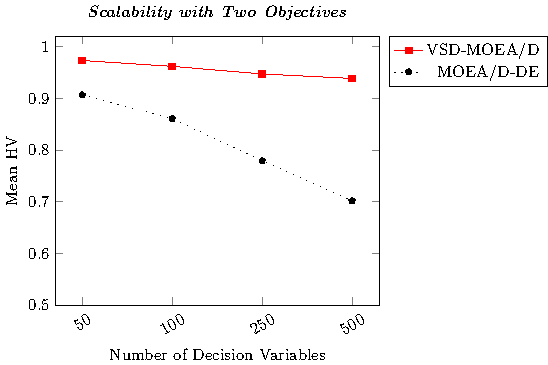
\includegraphics[scale=0.85]{images/Graphic-Scalability-2obj_tikz-figure0.eps}
\caption{Mean of the \HV{} ratio for 35 runs for the two-objective problems considering different numbers of variables}\label{fig:variable-decision-scalability-2obj}
\end{figure}

\begin{figure}[t]
\centering
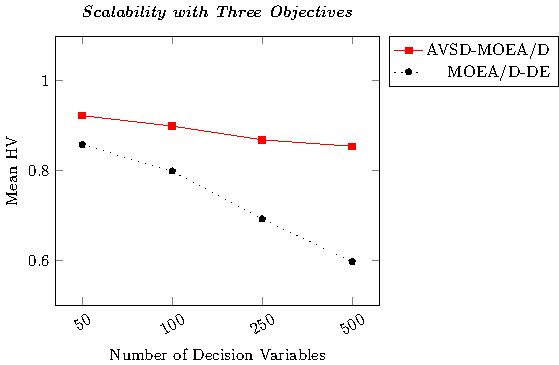
\includegraphics[scale=0.85]{images/Graphic-Scalability-3obj_tikz-figure0.eps}
\caption{Mean of the \HV{} ratio for 35 runs for the three-objective problems considering different numbers of variables} \label{fig:variable-decision-scalability-3obj}
\end{figure}

